\documentclass[12pt,a4paper]{article}

% ========== PACOTES ==========
\usepackage[utf8]{inputenc}
\usepackage[T1]{fontenc}
\usepackage[brazilian]{babel}
\usepackage{amsmath,amssymb,amsthm}
\usepackage{graphicx}
\usepackage[dvipsnames]{xcolor}
\usepackage{hyperref}
\usepackage{natbib}
\usepackage{geometry}
\usepackage{setspace}
\usepackage{enumitem}
\usepackage{booktabs}
\usepackage{longtable}
\usepackage{float}
\usepackage{caption}
\usepackage{footnote}
\usepackage{tcolorbox}
\usepackage{listings}
\usepackage{fancyhdr}
\usepackage{titlesec}
\usepackage{tocloft}
\usepackage{multicol}

% ========== GEOMETRIA ==========
\geometry{a4paper, left=2.5cm, right=2.5cm, top=2.5cm, bottom=2.5cm}
\onehalfspacing

% ========== CORES ==========
\definecolor{clearblue}{RGB}{27,58,92}
\definecolor{clearlightblue}{RGB}{44,95,138}
\definecolor{salmonbg}{RGB}{252,235,230}
\definecolor{salmonframe}{RGB}{230,160,140}
\definecolor{bluebg}{RGB}{235,245,251}
\definecolor{blueframe}{RGB}{58,125,181}
\definecolor{orangebg}{RGB}{254,245,231}
\definecolor{orangeframe}{RGB}{230,126,34}
\definecolor{codebg}{RGB}{248,248,248}
\definecolor{codeframe}{RGB}{200,200,200}
\definecolor{Rblue}{RGB}{0,80,160}
\definecolor{Rgreen}{RGB}{0,128,0}
\definecolor{Rgray}{RGB}{128,128,128}

% ========== HYPERREF ==========
\hypersetup{
  colorlinks=true, linkcolor=clearlightblue, citecolor=clearlightblue, urlcolor=clearlightblue,
  pdfauthor={FGV CLEAR},
  pdftitle={Avaliação de Impacto: Método de Controle Sintético (SCM)}
}

% ========== CABEÇALHOS ==========
\pagestyle{fancy}
\fancyhf{}
\fancyhead[R]{\small\textit{Guia CLEAR $|$ Controle Sintético (SCM)}}
\fancyfoot[C]{\thepage}
\renewcommand{\headrulewidth}{0pt}

% ========== TÍTULOS ==========
\titleformat{\section}{\Large\bfseries\color{clearblue}}{\thesection}{1em}{}
\titleformat{\subsection}{\large\bfseries\color{clearlightblue}}{\thesubsection}{1em}{}
\titleformat{\subsubsection}{\normalsize\bfseries\color{clearlightblue}}{\thesubsubsection}{1em}{}
\titleformat{\paragraph}[runin]{\normalsize\bfseries\itshape\color{clearblue}}{}{}{}[.]

% ========== CAIXAS ==========
\newtcolorbox{hipotesebox}[1][Hipóteses]{
  colback=salmonbg, colframe=salmonframe, coltitle=black, fonttitle=\bfseries,
  title=#1, boxrule=0.5pt, arc=2pt, left=6pt, right=6pt, top=4pt, bottom=4pt
}
\newtcolorbox{exemplobox}[1][Exemplo]{
  colback=salmonbg, colframe=salmonframe, coltitle=black, fonttitle=\bfseries,
  title=#1, boxrule=0.5pt, arc=2pt, left=6pt, right=6pt, top=4pt, bottom=4pt
}
\newtcolorbox{notabox}[1][Nota]{
  colback=bluebg, colframe=blueframe, coltitle=white, fonttitle=\bfseries,
  title=#1, boxrule=0.5pt, arc=2pt, left=6pt, right=6pt, top=4pt, bottom=4pt
}
\newtcolorbox{conexaobox}{
  colback=orangebg, colframe=orangeframe, boxrule=0.5pt, arc=2pt,
  left=6pt, right=6pt, top=3pt, bottom=3pt
}

% ========== LISTINGS ==========
\lstdefinestyle{Rstyle}{
  language=R, backgroundcolor=\color{codebg}, frame=single, rulecolor=\color{codeframe},
  basicstyle=\small\ttfamily, keywordstyle=\color{Rblue}\bfseries,
  stringstyle=\color{Rgreen}, commentstyle=\color{Rgray}\itshape,
  numbers=none, breaklines=true, showstringspaces=false, tabsize=2,
  xleftmargin=6pt, xrightmargin=6pt, aboveskip=8pt, belowskip=8pt,
  literate={á}{{\'a}}1 {é}{{\'e}}1 {í}{{\'i}}1 {ó}{{\'o}}1 {ú}{{\'u}}1
           {ã}{{\~a}}1 {õ}{{\~o}}1 {ç}{{\c{c}}}1 {ê}{{\^e}}1 {â}{{\^a}}1 {ô}{{\^o}}1
           {Á}{{\'A}}1 {É}{{\'E}}1 {Í}{{\'I}}1 {Ú}{{\'U}}1
           {<-}{{$\leftarrow$}}2
}
\lstdefinestyle{Routput}{
  backgroundcolor=\color{codebg}, frame=single, rulecolor=\color{codeframe},
  basicstyle=\small\ttfamily\color{Rgray}, numbers=none, breaklines=true,
  showstringspaces=false, xleftmargin=6pt, xrightmargin=6pt,
  aboveskip=4pt, belowskip=8pt
}

% ========== TEOREMAS ==========
\newtheorem{definicao}{Definição}[section]
\newtheorem{proposicao}{Proposição}[section]

% ========== METADADOS DE FIGURAS E TABELAS ==========
\newcommand{\figmeta}[3]{%
  \par\vspace{4pt}%
  \begin{minipage}{\linewidth}%
  \footnotesize%
  \textbf{Fonte:} #1\\%
  \textbf{Elaboração:} #2%
  \ifx&#3&\else\\[1pt]\textbf{Nota:} #3\fi%
  \end{minipage}%
  \vspace{6pt}%
}

% ========== DOCUMENTO ==========
\begin{document}

% ==========================================
% CAPA
% ==========================================
\thispagestyle{empty}
\begin{center}
\vspace*{4cm}
{\Large\bfseries\color{clearlightblue} SÉRIE: AVALIAÇÃO NA PRÁTICA}
\vspace{1.5cm}

{\Huge\bfseries\color{clearblue} Avaliação de Impacto:\\[0.3cm]
Método de Controle\\[0.3cm]
Sintético (SCM)}

\vspace{2cm}
{\large FGV CLEAR $|$ FGV EESP $|$ Global Evaluation Initiative}

\vspace{0.5cm}
{\large [Mês/Ano]}

\vfill

\begin{abstract}
\noindent Este guia apresenta o método de controle sintético (SCM) e suas extensões recentes para avaliação de impacto de políticas públicas. O SCM é particularmente útil quando há uma única unidade tratada --- ou poucas --- e um conjunto de unidades de controle potenciais, com dados em painel. O guia cobre desde o SCM clássico de \cite{AbadieGardeazabal2003} e \cite{AbadieDiamondHainmueller2010,AbadieDiamondHainmueller2015} até extensões como o SCM Aumentado \citep{BenMichaelEtAl2021}, o Controle Sintético Generalizado \citep{Xu2017}, o \textit{Synthetic Difference-in-Differences} \citep{ArkhangelskyEtAl2021}, e métodos de controle sintético com adoção escalonada \citep{BenMichaelFellerRothstein2022,CattaneoFengPalombaTitiunik2025}. A replicação empírica avalia o impacto da Lei Seca brasileira (Lei~11.705/2008) sobre a mortalidade no trânsito, usando países latino-americanos como pool de doadores. Todos os exemplos incluem código completo em R.
\end{abstract}
\end{center}
\newpage

% ==========================================
% FICHA TÉCNICA
% ==========================================
\thispagestyle{empty}
\section*{Ficha Técnica}

\textbf{Organizadores:} [Nome 1], [Nome 2]

\textbf{Equipe técnica:} [Listar membros]

\vspace{1cm}

\noindent\textbf{Apresentação.} Este guia integra a série de publicações \textit{Avaliação na Prática}, desenvolvida pelo FGV CLEAR com o objetivo de ampliar o acesso a conhecimentos sobre monitoramento e avaliação com foco em políticas públicas.

Fundado em 2015, o FGV CLEAR tem se dedicado ao fortalecimento da cultura de gestão orientada por evidências no Brasil e em países lusófonos. Com sede na Escola de Economia de São Paulo da Fundação Getulio Vargas (FGV EESP), o FGV CLEAR atua como centro regional da Iniciativa CLEAR (\textit{Centers for Learning on Evaluation and Results}).

Saiba mais sobre o FGV CLEAR e acesse outras publicações em: \textbf{www.fgvclear.org}
\newpage

% ==========================================
% SUMÁRIO
% ==========================================
\tableofcontents
\newpage


% ==========================================
% SEÇÃO 1: INTRODUÇÃO E MOTIVAÇÃO
% ==========================================
\section{Introdução e Motivação}

\subsection{O Problema de Avaliação com Poucos Tratados}

Uma das perguntas mais frequentes em avaliação de políticas públicas é: \textit{qual teria sido o resultado se a política não tivesse sido implementada?} Quando uma intervenção é aplicada a muitas unidades --- por exemplo, um programa social oferecido a milhares de famílias ---, dispomos de métodos bem estabelecidos para construir grupos de controle: experimentos randomizados, \textit{matching}, diferença-em-diferenças.

Mas o que acontece quando a política é implementada em \textbf{nível agregado}, afetando uma única unidade --- um país, um estado, uma cidade? Esse é o caso de muitas das políticas públicas relevantes:
\begin{itemize}[leftmargin=1.5cm]
  \item A Lei Seca brasileira (2008), aplicada em nível nacional;
  \item A reunificação da Alemanha (1990);
  \item A Proposição 99 na Califórnia (1988), que criou um programa de controle do tabaco;
  \item Políticas estaduais de segurança pública, como as UPPs no Rio de Janeiro.
\end{itemize}

Nesses contextos, os métodos tradicionais enfrentam desafios sérios. O \textit{matching} requer um pool grande de unidades comparáveis; a diferença-em-diferenças (DiD) exige que o grupo de controle siga a mesma tendência temporal que o grupo tratado na ausência do tratamento --- a hipótese de \textbf{tendências paralelas} ---, que é difícil de justificar quando as unidades são poucos países ou estados heterogêneos.\footnote{O Guia de DiD desta série discute em detalhe os problemas que surgem quando a hipótese de tendências paralelas é violada, especialmente no contexto de DiD escalonado.} Além disso, a \textbf{inferência estatística} é particularmente desafiadora nesse contexto: com apenas uma unidade tratada, métodos assintóticos tradicionais não se aplicam, e é preciso recorrer a procedimentos alternativos como testes placebo (Seção~2.4) ou inferência conformal (Seção~4.1).

O SCM, desenvolvido especificamente para esses casos, não impõe a hipótese de tendências paralelas; contudo, ele também tem seus requisitos. Em particular, exige que a unidade tratada possa ser bem aproximada por uma combinação convexa das unidades de controle disponíveis --- o que requer um \textbf{pool de doadores} suficientemente amplo e diversificado.\footnote{O termo \textit{pool de doadores} (\textit{donor pool}) refere-se ao conjunto de unidades não tratadas que servem de base para construir o controle sintético. A riqueza desse pool é determinante para a qualidade do ajuste pré-tratamento.} Se o pool é muito pequeno ou muito homogêneo, o ajuste pré-tratamento pode ser insuficiente. Essa tensão entre o número de doadores disponíveis e a qualidade do contrafactual é um dos aspectos práticos mais importantes do método.

\begin{conexaobox}
\textcolor{orangeframe}{\textbf{$\hookrightarrow$ Conexão com outros guias:}} \textit{Ver Guia de Avaliação de Impacto (Vol.~1 e 2) --- Seção sobre métodos quasi-experimentais; Guia de DiD --- Seção 1 (Hipótese de tendências paralelas e suas limitações).}
\end{conexaobox}


\subsection{A Ideia Central do Controle Sintético}

A intuição do SCM é elegante. Em vez de escolher uma \textit{única} unidade de controle (por exemplo, usar a Argentina como controle para o Brasil), o método constrói um \textbf{controle sintético}: uma combinação ponderada de várias unidades não tratadas que, juntas, reproduzem o mais fielmente possível a trajetória da unidade tratada \textit{antes} da intervenção.

Suponha que queremos avaliar o impacto da Lei Seca no Brasil. O SCM buscaria pesos $w_1, w_2, \ldots, w_J$ para países como Argentina, Chile, Colômbia, México, Peru, etc., de modo que:
\begin{equation}
  \text{Brasil Sintético}_t = w_1 \cdot Y_{\text{Argentina},t} + w_2 \cdot Y_{\text{Chile},t} + \cdots + w_J \cdot Y_{\text{Peru},t}
\end{equation}
reproduza a trajetória de mortalidade no trânsito do Brasil \textit{antes} de 2008. Se o ajuste pré-tratamento for bom, a trajetória do controle sintético \textit{depois} de 2008 serve como estimativa do contrafactual --- o que teria acontecido ao Brasil sem a Lei Seca. A diferença entre o Brasil real e o Brasil sintético é a estimativa do efeito causal.

\cite{AtheyImbens2017} descreveram o SCM como ``sem dúvida a inovação mais importante na literatura de avaliação de políticas dos últimos 15 anos''. O método tem três \textbf{propriedades} que o tornam especialmente atraente como ferramenta de análise:

\begin{enumerate}[leftmargin=1.5cm]
  \item \textbf{Transparência:} os pesos são explícitos --- sabemos exatamente quais unidades compõem o controle e com que peso;
  \item \textbf{Diagnóstico visual:} podemos verificar graficamente se o controle sintético replica bem a trajetória pré-tratamento;
  \item \textbf{Sem extrapolação:} a restrição de pesos não-negativos que somam 1 garante que o contrafactual está no suporte dos dados (combinação convexa).
\end{enumerate}

Essas são \textit{vantagens} do método --- o que o SCM oferece quando bem aplicado. Mas o SCM também possui \textbf{condições necessárias}: exige um período pré-tratamento suficientemente longo, um pool de doadores adequado, e que a unidade tratada esteja no fecho convexo das unidades de controle. Essas condições são formalizadas na Seção~2.2.

\begin{figure}[H]
\centering
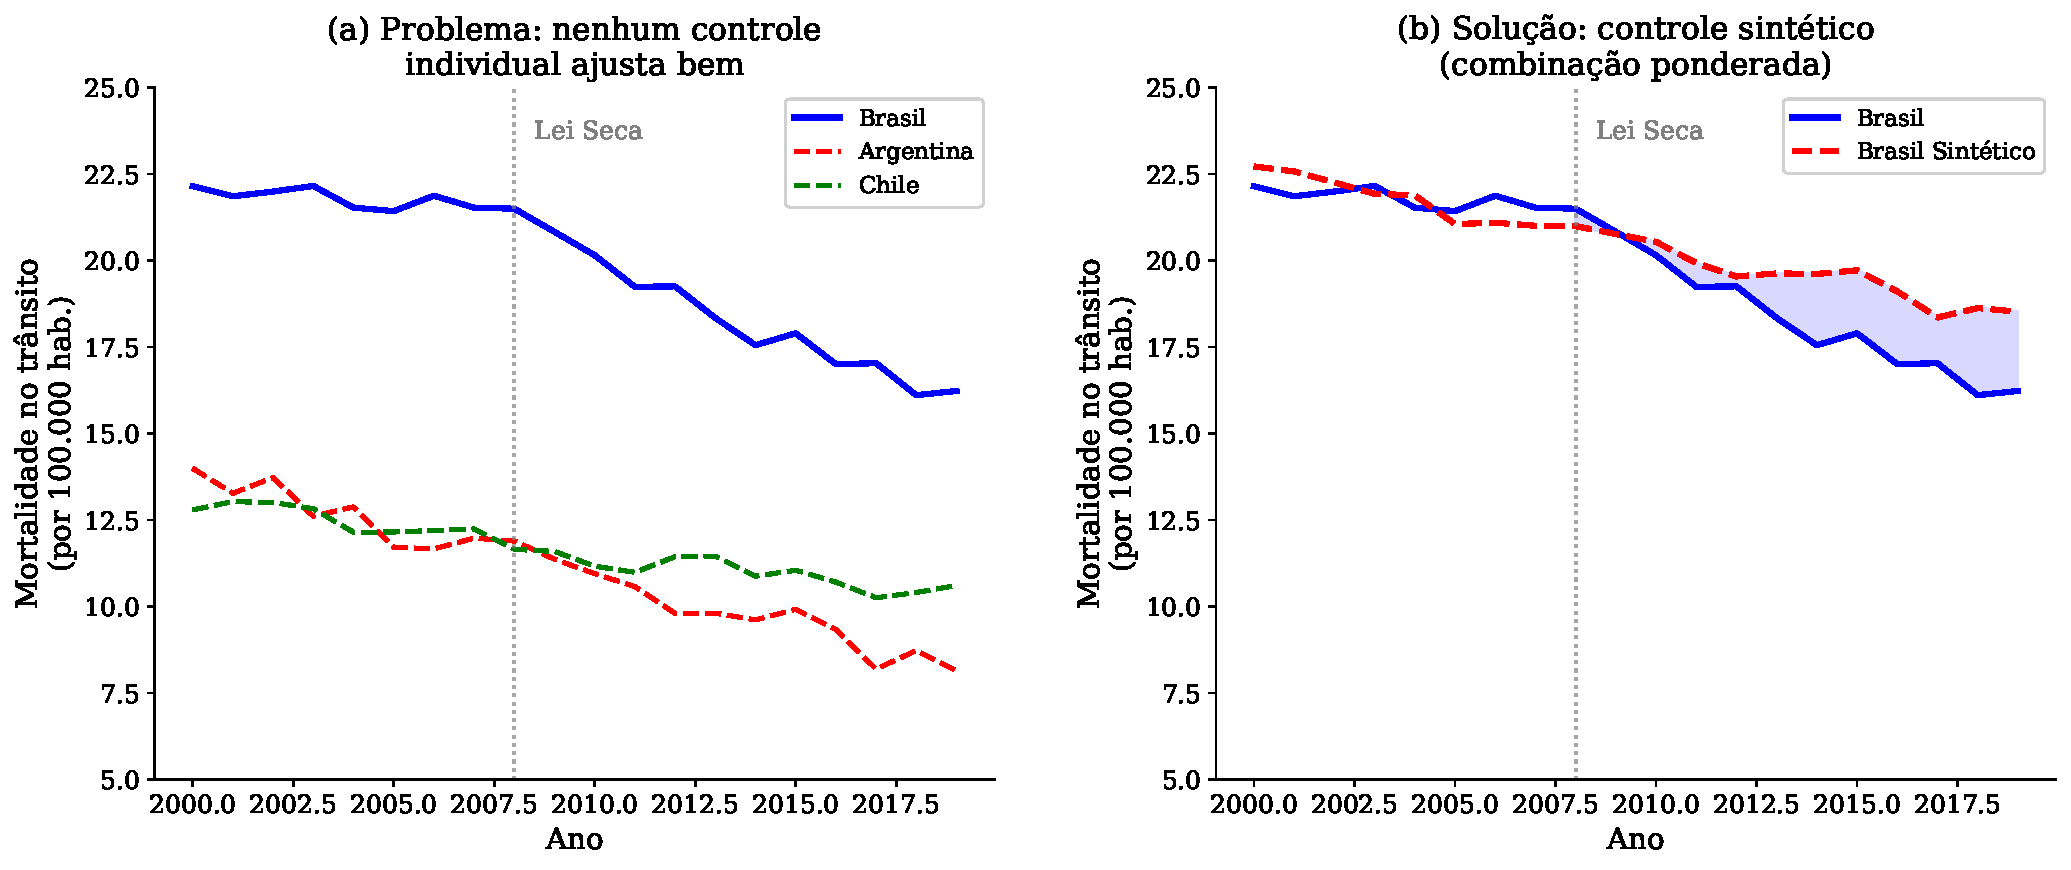
\includegraphics[width=\textwidth]{fig1_intuicao_scm.pdf}
\caption{Intuição do controle sintético}
\label{fig:intuicao}
\figmeta{Dados simulados com base em WHO/World Bank.}{FGV CLEAR.}{(a) Nenhum país individualmente replica a trajetória do Brasil. (b) Uma combinação ponderada (o ``Brasil Sintético'') ajusta bem o pré-tratamento; a diferença pós-tratamento estima o efeito.}
\end{figure}

A Figura~\ref{fig:intuicao} ilustra a intuição central do SCM. No painel (a), vemos que nem a Argentina nem o Chile, individualmente, replicam a trajetória de mortalidade no trânsito do Brasil --- ambos têm níveis e tendências muito diferentes. No painel (b), uma combinação ponderada de vários países constrói um ``Brasil Sintético'' que ajusta bem o período pré-tratamento; após 2008, a diferença entre o Brasil real e o sintético estima o efeito causal da Lei Seca.

\begin{conexaobox}
\textcolor{orangeframe}{\textbf{$\hookrightarrow$ Conexão com outros guias:}} \textit{Ver Guia de DiD --- Seção 1 (Comparação: SCM não requer a hipótese de tendências paralelas); Guia de Matching --- Seção 3 (Pareamento como construção de contrafactuais; SCM como extensão do matching para painel).}
\end{conexaobox}


\subsection{Exemplos Canônicos}

Três estudos seminais popularizaram o SCM e servem como referências metodológicas:

\paragraph{País Basco (Abadie e Gardeazabal, 2003)} O primeiro artigo a propor o SCM avaliou o impacto econômico do terrorismo do ETA no País Basco, comparando seu PIB per capita com um ``País Basco Sintético'' construído a partir de outras regiões espanholas. Os autores mostraram que o conflito reduziu o PIB per capita do País Basco em aproximadamente 10 pontos percentuais \citep{AbadieGardeazabal2003}.

\paragraph{Proposição 99 na Califórnia (Abadie, Diamond e Hainmueller, 2010)} O artigo que formalizou o SCM avaliou o efeito do programa de controle do tabaco da Califórnia (1988) sobre as vendas de cigarro per capita. Usando outros estados americanos como doadores, os autores estimaram uma redução significativa nas vendas após a implementação do programa --- um resultado que se tornou o exemplo didático padrão do método \citep{AbadieDiamondHainmueller2010}.

\paragraph{Reunificação Alemã (Abadie, Diamond e Hainmueller, 2015)} A reunificação alemã de 1990 é um caso paradigmático de intervenção em nível nacional. Os autores estimaram que a reunificação reduziu o PIB per capita da Alemanha Ocidental em aproximadamente 1.600 dólares por ano até 2003 \citep{AbadieDiamondHainmueller2015}. Esse artigo também formalizou os testes placebo \textit{in-space} e \textit{in-time} como ferramentas de inferência.

\paragraph{Zona Franca de Manaus (Possebom, 2019)} No contexto brasileiro, \cite{Possebom2019} aplica o SCM para avaliar os efeitos econômicos da Zona Franca de Manaus. Usando outros estados brasileiros como pool de doadores, o autor constrói um ``Amazonas Sintético'' e estima o impacto dos incentivos fiscais sobre o desenvolvimento econômico regional --- uma contribuição importante ao debate sobre a efetividade de políticas de desenvolvimento baseadas em zonas de livre comércio no Brasil.

\begin{notabox}[Figuras dos estudos canônicos]
Os gráficos de trajetória (\textit{path plot}) e de gap (\textit{gap plot}) dos três estudos acima são referências visuais essenciais para qualquer praticante do SCM. Recomendamos fortemente consultar as figuras originais em \cite{AbadieGardeazabal2003}, \cite{AbadieDiamondHainmueller2010} e \cite{AbadieDiamondHainmueller2015}, que ilustram com clareza o ajuste pré-tratamento e a divergência pós-intervenção que fundamentam a interpretação causal.
\end{notabox}


\subsection{SCM no Ecossistema de Métodos de Avaliação}

Para situar o SCM em relação aos demais métodos, a Tabela~\ref{tab:ecossistema} apresenta uma comparação das principais características.

\begin{table}[H]
\centering
\caption{Comparação do SCM com outros métodos de avaliação de impacto}
\label{tab:ecossistema}
\small
\begin{tabular}{lcccc}
\toprule
\textbf{Característica} & \textbf{DiD} & \textbf{Matching} & \textbf{RDD} & \textbf{SCM} \\
\midrule
Múltiplos tratados     & Sim           & Sim             & Sim          & Não (padrão)$^\dagger$ \\
Poucos tratados        & Difícil       & Difícil         & N/A          & \textbf{Ideal} \\
Tend.\ paralelas       & Requer        & Não requer      & Não requer   & Não requer \\
Transparência          & Média         & Alta            & Alta         & \textbf{Muito alta} \\
Dados em painel        & Requer        & Opcional        & Não requer   & Requer \\
Validade               & Global$^*$    & Global$^*$      & Local        & Local (à unidade) \\
\bottomrule
\multicolumn{5}{l}{\footnotesize $^\dagger$ Extensões (GSC, Staggered SCM) permitem múltiplos tratados.} \\
\multicolumn{5}{l}{\footnotesize $^*$ Condicional às hipóteses de identificação.} \\
\multicolumn{5}{l}{\footnotesize \textbf{Elaboração:} FGV CLEAR.}
\end{tabular}
\end{table}

\begin{conexaobox}
\textcolor{orangeframe}{\textbf{$\hookrightarrow$ Conexão com outros guias:}} \textit{Ver Guia de RDD --- Seção 1.3 (RDD no ecossistema); Guia de Matching --- Seção 1 (Arcabouço causal geral).}
\end{conexaobox}

\subsection{Por Que Não Usar DiD? O Problema das Tendências Paralelas}

Uma pergunta natural é: por que não simplesmente usar diferença-em-diferenças? A Figura~\ref{fig:did_vs_scm} ilustra o problema. Quando as tendências pré-tratamento são paralelas entre tratado e controle (painel a), o DiD identifica corretamente o efeito causal. Mas quando as tendências divergem (painel b) --- o que é comum quando as unidades são países ou estados heterogêneos ---, o contrafactual do DiD é enviesado. O SCM (painel c) resolve isso buscando pesos que \textit{ajustam} a trajetória pré-tratamento, não apenas o nível.

\begin{figure}[H]
\centering
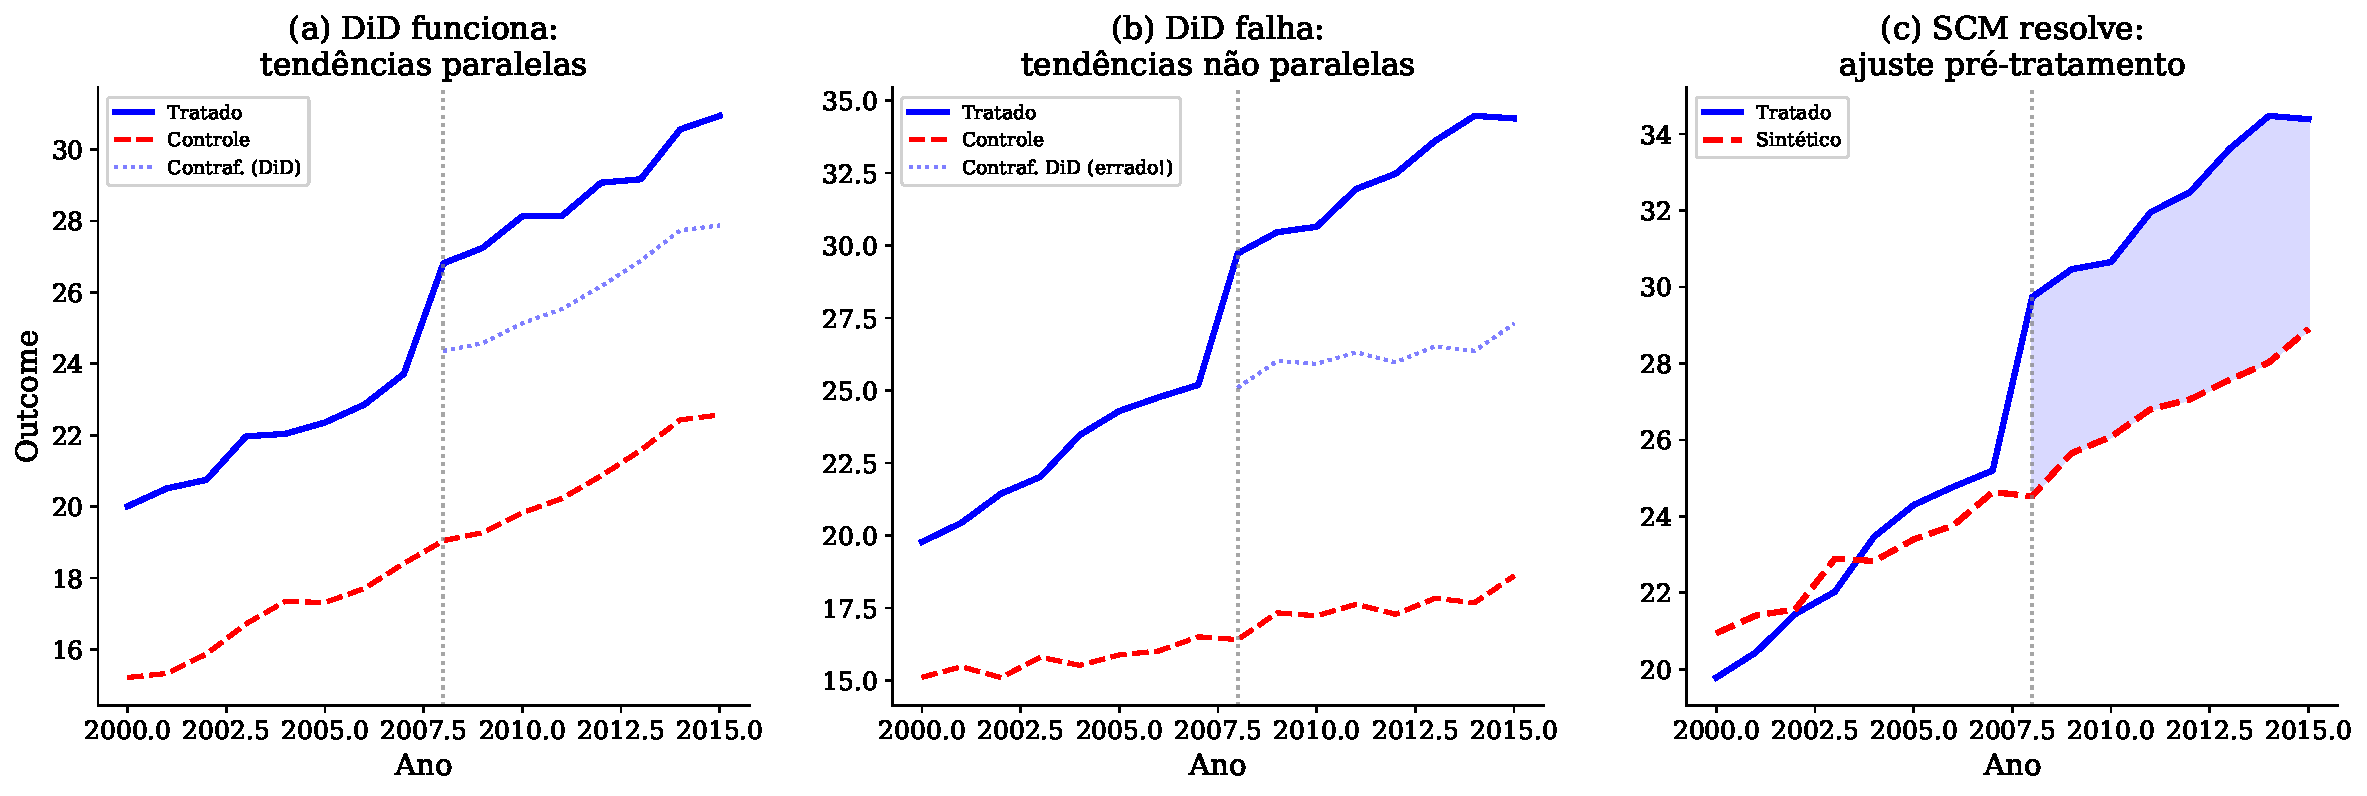
\includegraphics[width=\textwidth]{fig4_did_vs_scm.pdf}
\caption{Comparação: quando o DiD falha e o SCM resolve}
\label{fig:did_vs_scm}
\figmeta{Dados simulados.}{FGV CLEAR.}{(a) Com tendências paralelas, o DiD identifica o efeito. (b) Sem tendências paralelas, o contrafactual do DiD é enviesado. (c) O SCM busca pesos que replicam a trajetória pré-tratamento.}
\end{figure}

A Figura~\ref{fig:did_vs_scm} ilustra por que o SCM é preferível ao DiD em muitos contextos comparativos. Quando as tendências pré-tratamento entre tratado e controle são paralelas (painel a), o DiD funciona bem. Porém, quando as tendências divergem --- situação comum quando as unidades são países ou estados heterogêneos --- o contrafactual do DiD extrapola erroneamente (painel b). O SCM resolve esse problema buscando pesos que ajustam a trajetória, não apenas o nível (painel c).

Essa comparação revela uma complementaridade fundamental: o DiD é robusto a diferenças \textit{permanentes} de nível entre unidades (via efeitos fixos), enquanto o SCM é robusto a diferenças na \textit{dinâmica temporal} (via ajuste de trajetória). O SDID (Seção~3.5) combina ambas as vantagens.

\begin{conexaobox}
\textcolor{orangeframe}{\textbf{$\hookrightarrow$ Conexão com outros guias:}} \textit{Ver Guia de DiD --- Seção 1 (Hipótese de tendências paralelas e testes de pré-tendência); Guia de Matching --- Seção 2 (Hipótese de seleção em observáveis vs não-observáveis).}
\end{conexaobox}



% ==========================================
% SEÇÃO 2: ARCABOUÇO TEÓRICO
% ==========================================
\newpage
\section{Arcabouço Teórico}

Nesta seção, desenvolvemos formalmente o SCM, partindo do modelo de resultados potenciais até chegar ao estimador e suas propriedades. Seguimos de perto a formalização de \cite{AbadieDiamondHainmueller2010} e \cite{Abadie2021}, adaptando a notação ao padrão dos guias desta série.

\subsection{Modelo de Resultados Potenciais e o Modelo Fatorial}

Considere $J+1$ unidades observadas por $T$ períodos. A unidade $j=1$ recebe tratamento a partir do período $T_0 + 1$; as unidades $j = 2, \ldots, J+1$ não recebem tratamento em nenhum período (o ``pool de doadores''). Portanto, os períodos $t = 1, \ldots, T_0$ constituem o \textbf{período pré-tratamento}, e os períodos $t = T_0 + 1, \ldots, T$ constituem o \textbf{período pós-tratamento}. Em particular, $T_0$ é o \textit{último} período antes do tratamento --- não o número de períodos pré-tratamento, embora os dois coincidam quando o painel começa em $t=1$.\footnote{Por exemplo, se o painel cobre 2000--2019 e o tratamento começa em 2008, então $T_0$ corresponde a 2007, e há 8 períodos pré-tratamento ($T_0 = 8$ se indexarmos a partir de 1).}

Para cada unidade $j$ e período $t$, definimos os resultados potenciais $Y_{jt}(0)$ (sem tratamento) e $Y_{jt}(1)$ (com tratamento). O efeito causal do tratamento sobre a unidade tratada no período $t > T_0$ é:
\begin{equation}
  \tau_{1t} = Y_{1t}(1) - Y_{1t}(0).
  \label{eq:tau}
\end{equation}
Observamos $Y_{1t}(1)$ para $t > T_0$, mas não observamos $Y_{1t}(0)$ --- esse é o contrafactual que precisamos estimar.

O modelo fatorial linear de \cite{AbadieDiamondHainmueller2010} especifica o resultado potencial sem tratamento como:
\begin{equation}
  Y_{jt}(0) = \delta_t + \boldsymbol{\theta}_t' \mathbf{Z}_j + \boldsymbol{\lambda}_t' \boldsymbol{\mu}_j + \varepsilon_{jt},
  \label{eq:factor_model}
\end{equation}
onde:
\begin{itemize}[leftmargin=1.5cm]
  \item $\delta_t$ é um efeito fixo de tempo comum a todas as unidades;
  \item $\mathbf{Z}_j$ é um vetor $(r \times 1)$ de covariáveis observadas (não afetadas pelo tratamento);
  \item $\boldsymbol{\theta}_t$ são os coeficientes variantes no tempo dessas covariáveis;
  \item $\boldsymbol{\mu}_j$ é um vetor $(F \times 1)$ de \textbf{fatores latentes} não observados, específicos de cada unidade;
  \item $\boldsymbol{\lambda}_t$ é um vetor $(F \times 1)$ de \textit{factor loadings} variantes no tempo;
  \item $\varepsilon_{jt}$ é um erro idiossincrático com $E[\varepsilon_{jt}] = 0$.
\end{itemize}

\begin{notabox}[Por que o modelo fatorial?]
O modelo fatorial é mais geral que o modelo de efeitos fixos aditivos usado na diferença-em-diferenças. No DiD, assumimos $Y_{jt}(0) = \alpha_j + \gamma_t + \varepsilon_{jt}$, onde os efeitos fixos de unidade $\alpha_j$ são \textit{constantes} no tempo. O modelo fatorial permite que os efeitos não observados $\boldsymbol{\mu}_j$ interajam com os \textit{factor loadings} $\boldsymbol{\lambda}_t$ de maneira variante no tempo. Isso é crucial: é o que permite ao SCM funcionar sem a hipótese de tendências paralelas.
\end{notabox}

\begin{conexaobox}
\textcolor{orangeframe}{\textbf{$\hookrightarrow$ Conexão com outros guias:}} \textit{Ver Guia de DiD --- Seção 1.1 (Modelo de resultados potenciais e a importância de definir bem o estimando); Seção 2 (DiD escalonado e modelo fatorial; relação com TWFE).}
\end{conexaobox}


\subsection{O Resultado Central: Por Que o SCM Funciona}

A pergunta-chave é: se encontrarmos pesos $\mathbf{w}^* = (w_2^*, \ldots, w_{J+1}^*)'$ que reproduzem perfeitamente os resultados pré-tratamento, esses pesos também reproduzem o contrafactual pós-tratamento?

A Proposição 1 de \cite{AbadieDiamondHainmueller2010} responde afirmativamente, sob condições. Suponha que existam pesos $w_2^*, \ldots, w_{J+1}^*$ com $w_j^* \geq 0$ e $\sum_j w_j^* = 1$ tais que:
\begin{equation}
  \sum_{j=2}^{J+1} w_j^* Y_{jt} = Y_{1t} \quad \text{para todo} \quad t = 1, \ldots, T_0
  \label{eq:perfect_fit}
\end{equation}
e
\begin{equation}
  \sum_{j=2}^{J+1} w_j^* \mathbf{Z}_j = \mathbf{Z}_1.
  \label{eq:cov_balance}
\end{equation}

Então, se $T_0$ é ``grande o suficiente'' em relação à escala dos erros transitórios $\varepsilon_{jt}$, temos que:\footnote{Formalmente, o viés é limitado e converge a zero quando $T_0 \to \infty$ sob condições de regularidade. Ver \cite{Abadie2021}, Seção 3.2, para uma discussão detalhada.}
\begin{equation}
  Y_{1t}(0) \approx \sum_{j=2}^{J+1} w_j^* Y_{jt} \quad \text{para} \quad t > T_0.
\end{equation}

A intuição é poderosa: se os pesos reproduzem simultaneamente as covariáveis observadas $\mathbf{Z}_1$ e toda a trajetória pré-tratamento $Y_{1,1}, \ldots, Y_{1,T_0}$, então eles \textit{implicitamente} reproduzem também os fatores latentes $\boldsymbol{\mu}_1$. Isso acontece porque os outcomes pré-tratamento são funções dos fatores latentes, e com $T_0$ períodos suficientes, há informação bastante para ``identificar'' $\boldsymbol{\mu}_1$ através da combinação linear dos doadores.

\begin{hipotesebox}[Condições para o Resultado Central]
\begin{enumerate}
  \item \textbf{Modelo fatorial:} $Y_{jt}(0)$ segue a Equação~\eqref{eq:factor_model};
  \item \textbf{Ajuste perfeito pré-tratamento:} existem pesos que satisfazem \eqref{eq:perfect_fit} e \eqref{eq:cov_balance};
  \item \textbf{$T_0$ suficientemente grande:} o número de períodos pré-tratamento domina a variação dos erros transitórios;
  \item \textbf{Interpolação:} a unidade tratada está no fecho convexo das unidades de controle.
\end{enumerate}
\end{hipotesebox}


\subsection{O Estimador SCM Clássico}

\subsubsection{Formulação do Problema de Otimização}

Na prática, o ajuste perfeito \eqref{eq:perfect_fit} raramente é possível. O estimador SCM busca pesos que \textit{minimizam} a distância entre os preditores da unidade tratada e o controle sintético:

\begin{equation}
  \mathbf{w}^* = \arg\min_{\mathbf{w}} \|\mathbf{X}_1 - \mathbf{X}_0 \mathbf{w}\|_{\mathbf{V}} \quad \text{sujeito a} \quad w_j \geq 0, \quad \sum_{j=2}^{J+1} w_j = 1,
  \label{eq:scm_opt}
\end{equation}
onde:
\begin{itemize}[leftmargin=1.5cm]
  \item $\mathbf{X}_1$ é um vetor $(k \times 1)$ de preditores da unidade tratada (médias pré-tratamento de covariáveis e outcomes);
  \item $\mathbf{X}_0$ é uma matriz $(k \times J)$ de preditores das unidades de controle;
  \item $\mathbf{V}$ é uma matriz $(k \times k)$ simétrica e positiva semi-definida que pondera a importância relativa de cada preditor;
  \item $\|\mathbf{a}\|_{\mathbf{V}} = (\mathbf{a}'\mathbf{V}\mathbf{a})^{1/2}$.
\end{itemize}

\subsubsection{A Escolha da Matriz de Pesos V}

A escolha de $\mathbf{V}$ é uma decisão importante. As abordagens mais comuns são:

\begin{enumerate}[leftmargin=1.5cm]
  \item \textbf{Cross-validation:} escolher $\mathbf{V}$ que minimiza o RMSPE\footnote{RMSPE = \textit{Root Mean Squared Prediction Error}: $\text{RMSPE} = \sqrt{\frac{1}{T_0} \sum_{t=1}^{T_0} (Y_{1t} - \sum_j w_j^* Y_{jt})^2}$.} pré-tratamento, dividindo o período pré em treino e validação;
  \item \textbf{Minimização direta:} resolver um problema aninhado (nested) que escolhe $\mathbf{V}$ para minimizar o RMSPE pré-tratamento --- esta é a abordagem padrão do pacote \texttt{Synth};
  \item \textbf{Inversa da variância:} usar $\mathbf{V} = \text{diag}(1/\hat{\sigma}_k^2)$, ponderando cada preditor pelo inverso de sua variância amostral.
\end{enumerate}

\subsubsection{Propriedades dos Pesos}

Os pesos $w_j^*$ possuem propriedades importantes:
\begin{itemize}[leftmargin=1.5cm]
  \item \textbf{Esparsidade:} tipicamente, poucos doadores recebem peso positivo --- \cite{Abadie2021} mostra que, sob unicidade da solução, o número de pesos positivos é limitado pelo número de preditores $k$;
  \item \textbf{Não-negatividade e soma 1:} garantem interpolação (não extrapolação), fundamentando a interpretação do controle sintético como ``média ponderada'' de unidades reais;
  \item \textbf{Transparência:} os pesos são interpretáveis --- podemos inspecionar quais unidades compõem o contrafactual e com que importância.
\end{itemize}

\begin{notabox}[Esparsidade como diagnóstico]
A esparsidade dos pesos pode ser informativa. Se muitas unidades recebem peso positivo com valores similares, isso sugere que nenhuma combinação é realmente boa --- o contrafactual é construído ``na média''. Se poucos doadores concentram a maior parte do peso, a analogia com matching se torna mais direta e a interpretabilidade aumenta.
\end{notabox}


\subsubsection{O Estimador do Efeito Causal}

Dados os pesos ótimos $\mathbf{w}^*$, o efeito causal estimado para a unidade tratada no período $t > T_0$ é:
\begin{equation}
  \hat{\tau}_{1t} = Y_{1t} - \sum_{j=2}^{J+1} w_j^* Y_{jt}.
  \label{eq:effect}
\end{equation}

O \textit{gap} (diferença) entre a unidade tratada e o controle sintético ao longo do tempo é a quantidade central de interesse, tipicamente representada no ``gap plot''.


\subsubsection{Código em R: Exemplo com a Proposição 99}

Demonstramos a implementação com o pacote \texttt{Synth}, replicando o estudo clássico da Califórnia. Este exemplo é particularmente adequado do ponto de vista didático: o controle sintético replica a trajetória pré-tratamento com precisão quase perfeita, tornando visualmente inequívoca a divergência pós-1988. Casos com ajuste pré-tratamento excelente são os mais fáceis de interpretar e servem como referência para avaliar a qualidade de outras aplicações.\footnote{Na prática, nem sempre é possível obter um ajuste tão bom quanto no exemplo da Califórnia. A Seção~3.1 discute o ASCM, que corrige o viés quando o ajuste pré-tratamento é imperfeito.}

\begin{lstlisting}[style=Rstyle]
# Instalação e carregamento
install.packages("Synth")
library(Synth)

# Dados: vendas de cigarro per capita por estado, 1970-2000
# NOTA: O dataset "synth.data" do pacote Synth é um conjunto simulado
# para exemplos genéricos. Para replicar o exemplo da Califórnia
# (Proposição 99), use os dados disponíveis em:
#   https://web.stanford.edu/~jhain/synthpage.html
# Abaixo, assumimos que o dataset foi carregado como "smoking",
# que contém: state, year, cigsale, lnincome, beer, age15to24, retprice
# (note: a variável de renda chama-se "lnincome", não "income")

# Preparação dos dados
dataprep.out <- dataprep(
  foo = smoking,
  predictors = c("lnincome", "retprice", "age15to24"),
  predictors.op = "mean",
  dependent = "cigsale",
  unit.variable = "unit.num",
  time.variable = "year",
  treatment.identifier = 3,         # California
  controls.identifier = c(2, 4:39), # demais estados
  time.predictors.prior = 1980:1988,
  time.optimize.ssr = 1980:1988,
  time.plot = 1970:2000
)

# Estimação dos pesos ótimos
synth.out <- synth(dataprep.out)

# Tabela de pesos: quais estados compõem a Califórnia Sintética?
synth.tables <- synth.tab(dataprep.res = dataprep.out,
                          synth.res = synth.out)
print(synth.tables$tab.w)  # pesos por estado
print(synth.tables$tab.v)  # pesos dos preditores (V)
print(synth.tables$tab.pred) # comparação de preditores

# Gráfico de trajetória (path plot)
path.plot(synth.res = synth.out,
          dataprep.res = dataprep.out,
          Ylab = "Vendas de cigarro per capita (maços)",
          Xlab = "Ano",
          Legend = c("Califórnia", "Califórnia Sintética"),
          Legend.position = "bottomleft")
abline(v = 1988, lty = 2, col = "red")  # linha do tratamento

# Gap plot (efeito ao longo do tempo)
gaps.plot(synth.res = synth.out,
          dataprep.res = dataprep.out,
          Ylab = "Gap (Califórnia - Sintética)",
          Xlab = "Ano")
abline(v = 1988, lty = 2, col = "red")
abline(h = 0, lty = 3)
\end{lstlisting}

\begin{exemplobox}[Interpretação dos Resultados]
Na replicação da Proposição 99, a Califórnia Sintética é composta principalmente por Utah, Nevada e Connecticut, com pesos que refletem a similaridade dessas economias com a Califórnia no período pré-tratamento. O gap plot mostra que, a partir de 1988, as vendas de cigarro na Califórnia caem sistematicamente abaixo do controle sintético, sugerindo que o programa de controle do tabaco reduziu efetivamente o consumo. A estimativa do efeito acumulado até 2000 é de aproximadamente 25 maços per capita por ano.
\end{exemplobox}

\begin{figure}[H]
\centering
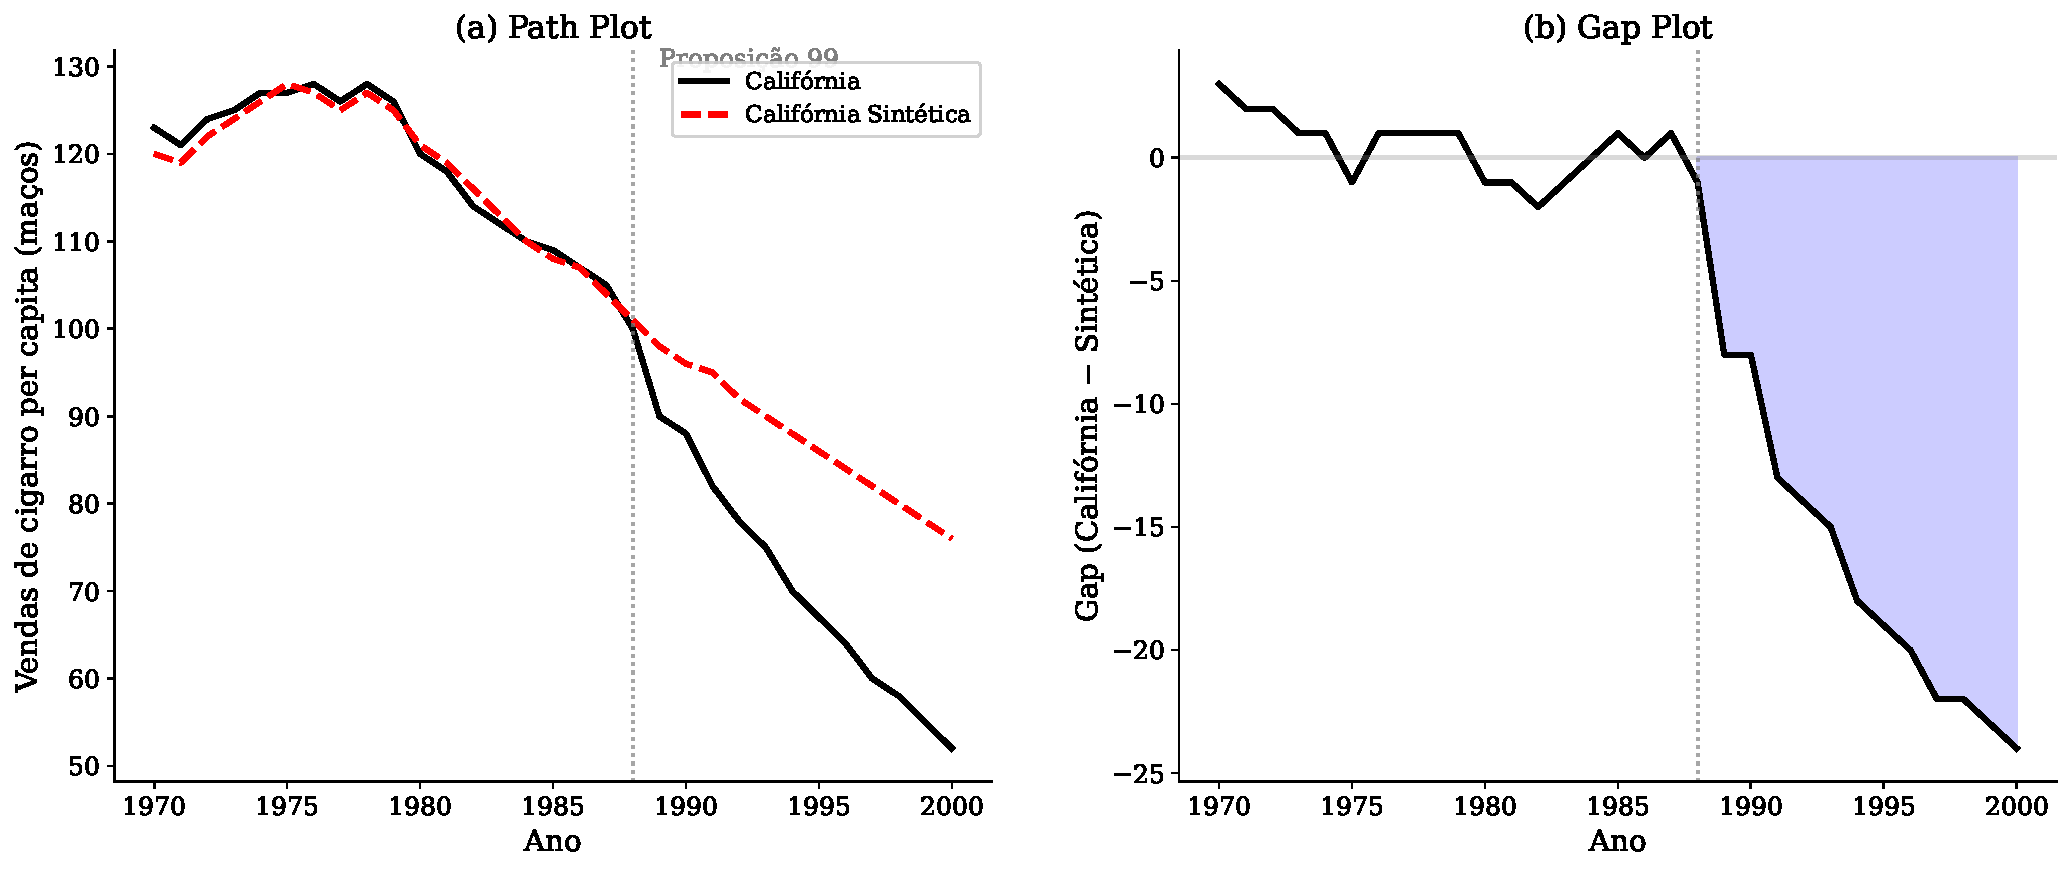
\includegraphics[width=\textwidth]{fig2_california_path_gap.pdf}
\caption{Proposição 99 na Califórnia: \textit{path plot} e \textit{gap plot}}
\label{fig:california}
\figmeta{Replicação de \cite{AbadieDiamondHainmueller2010} com dados do pacote \texttt{Synth}.}{FGV CLEAR.}{(a) A Califórnia Sintética replica bem a trajetória pré-1988. (b) O gap mostra efeito crescente, atingindo $\sim$25 maços per capita em 2000.}
\end{figure}

A Figura~\ref{fig:california} apresenta os dois gráficos fundamentais de qualquer análise SCM. O \textit{path plot} (painel a) mostra que a Califórnia Sintética --- construída a partir de outros estados americanos --- replica com excelente precisão a trajetória de vendas de cigarro pré-1988. Após a implementação da Proposição~99, as vendas na Califórnia real caem sistematicamente abaixo do contrafactual. O \textit{gap plot} (painel b) torna essa divergência mais clara: o efeito negativo cresce ao longo do tempo, indicando que o programa de controle do tabaco reduziu progressivamente o consumo.

A Tabela~\ref{tab:pesos_california} mostra os pesos estimados dos principais doadores. Note que a solução é esparsa: apenas 5 dos 38 estados do pool recebem peso positivo significativo.

\begin{table}[H]
\centering
\caption{Pesos dos principais doadores --- Califórnia Sintética}
\label{tab:pesos_california}
\small
\begin{tabular}{lc}
\toprule
\textbf{Estado} & \textbf{Peso} \\
\midrule
Utah            & 0.334 \\
Nevada          & 0.234 \\
Connecticut     & 0.199 \\
Montana         & 0.164 \\
Colorado        & 0.069 \\
\midrule
\textit{Demais (33 estados)} & 0.000 \\
\bottomrule
\multicolumn{2}{l}{\footnotesize \textbf{Fonte:} Replicação com pacote \texttt{Synth}. \textbf{Elaboração:} FGV CLEAR.}
\end{tabular}
\end{table}

\begin{conexaobox}
\textcolor{orangeframe}{\textbf{$\hookrightarrow$ Conexão com outros guias:}} \textit{Ver Guia de DiD --- Seção 3 (Padrões de código em R e boas práticas de replicação).}
\end{conexaobox}


\subsection{Inferência no SCM Clássico}

A inferência no SCM é, talvez, o aspecto mais delicado do método. Ao contrário de métodos com muitas unidades onde a teoria assintótica é natural, o SCM opera tipicamente com uma única unidade tratada e um pool modesto de doadores. Não há, em geral, distribuição assintótica do estimador à qual possamos recorrer.

\subsubsection{Testes Placebo In-Space}

O procedimento de inferência mais utilizado no SCM foi proposto por \cite{AbadieDiamondHainmueller2015}. A ideia é replicar a análise para \textit{cada} unidade do pool de doadores, como se ela fosse a tratada:

\begin{enumerate}[leftmargin=1.5cm]
  \item Para cada unidade $j = 2, \ldots, J+1$:
  \begin{enumerate}
    \item[(a)] Tratar $j$ como se fosse a unidade tratada;
    \item[(b)] Usar as demais unidades (incluindo a verdadeiramente tratada) como pool de doadores;
    \item[(c)] Estimar o ``efeito placebo'' $\hat{\tau}_{jt}^{\text{placebo}}$;
  \end{enumerate}
  \item Comparar o efeito estimado da unidade verdadeiramente tratada com a distribuição dos efeitos placebo;
  \item Se o efeito da unidade tratada é ``incomum'' em relação à distribuição placebo, há evidência de um efeito real.
\end{enumerate}

\begin{lstlisting}[style=Rstyle]
# Testes placebo in-space
# Loop sobre todas as unidades de controle
store <- matrix(NA, length(1970:2000), length(c(2, 4:39)))
colnames(store) <- c(2, 4:39)

for (i in c(2, 4:39)) {
  tryCatch({
    dataprep.placebo <- dataprep(
      foo = smoking,
      predictors = c("lnincome", "retprice", "age15to24"),
      predictors.op = "mean",
      dependent = "cigsale",
      unit.variable = "unit.num",
      time.variable = "year",
      treatment.identifier = i,
      controls.identifier = setdiff(c(2:39), i),
      time.predictors.prior = 1980:1988,
      time.optimize.ssr = 1980:1988,
      time.plot = 1970:2000
    )
    synth.placebo <- synth(dataprep.placebo)
    store[, as.character(i)] <-
      dataprep.placebo$Y1plot - (dataprep.placebo$Y0plot
        %*% synth.placebo$solution.w)
  }, error = function(e) { cat("Unidade", i, "falhou\n") })
}

# Gráfico: gaps da Califórnia (preto) vs placebos (cinza)
plot(1970:2000, store[, "3"], type = "l", lwd = 2,
     ylim = range(store, na.rm = TRUE),
     xlab = "Ano", ylab = "Gap (maços per capita)")
for (i in setdiff(colnames(store), "3")) {
  lines(1970:2000, store[, i], col = "grey70")
}
lines(1970:2000, store[, "3"], lwd = 2)  # Califórnia por cima
abline(v = 1988, lty = 2, col = "red")
abline(h = 0, lty = 3)
\end{lstlisting}

\subsubsection{Testes Placebo In-Time}

\begin{figure}[H]
\centering
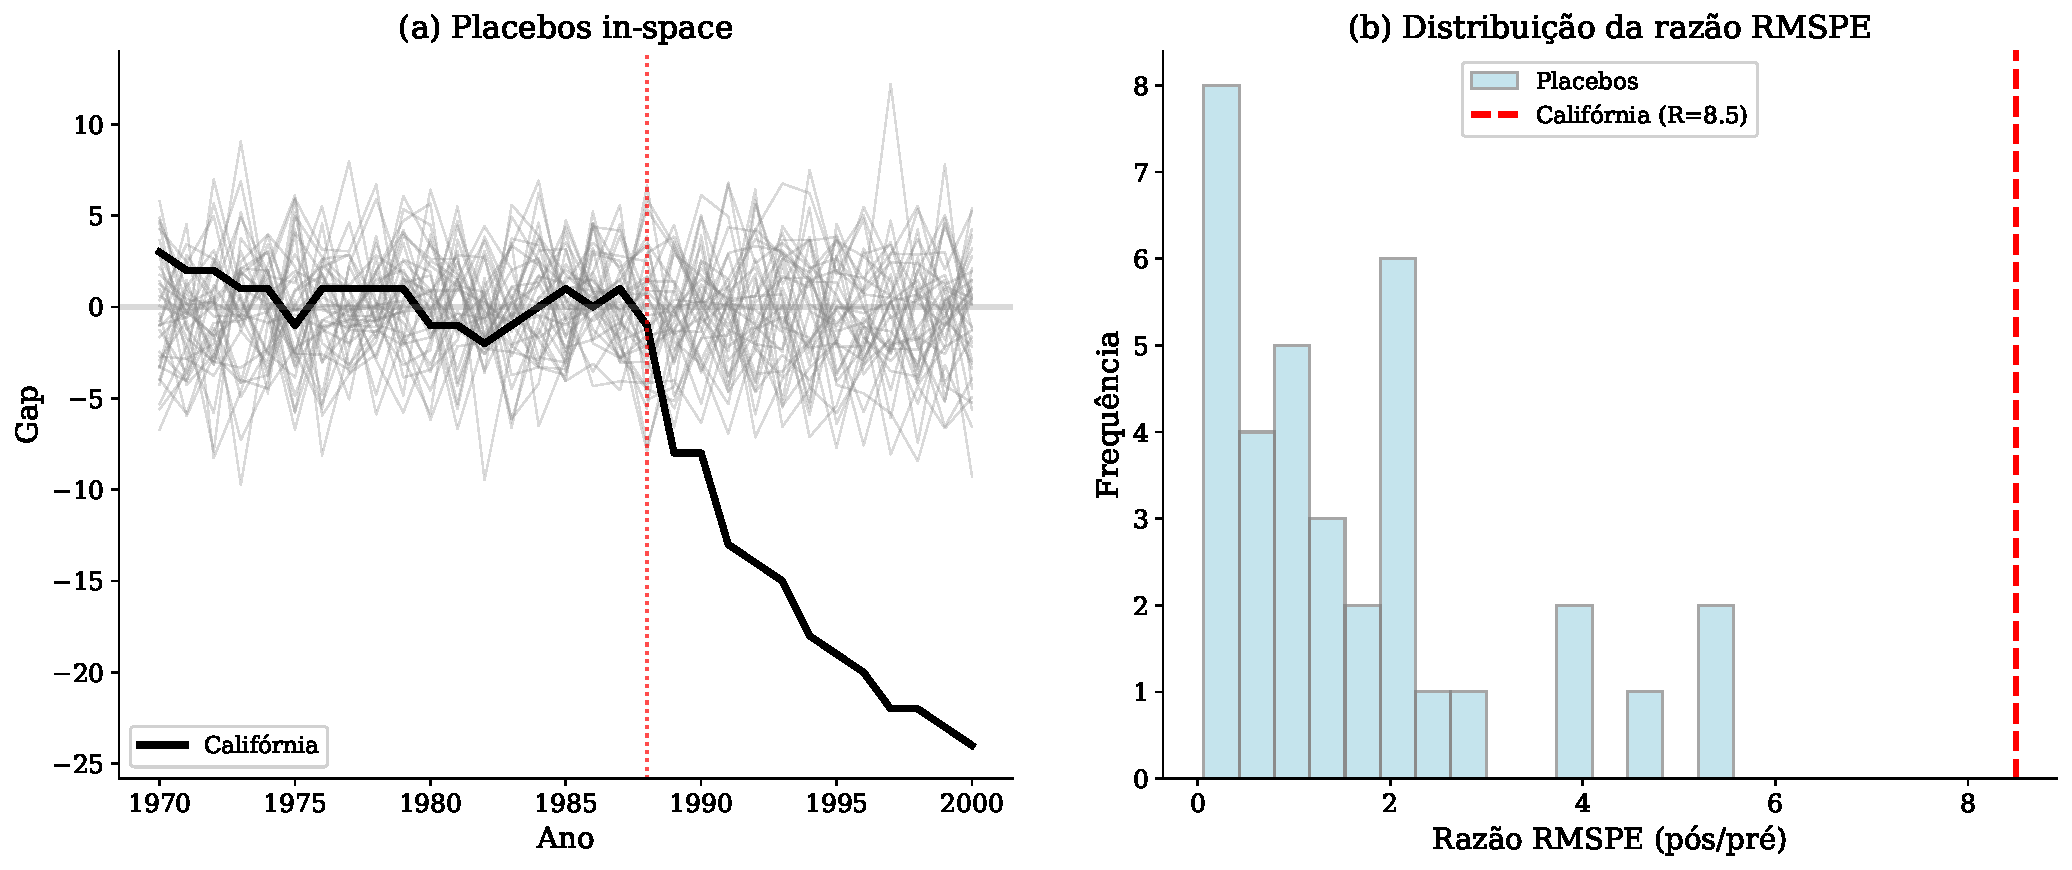
\includegraphics[width=\textwidth]{fig3_placebos.pdf}
\caption{Testes placebo in-space para a Proposição 99}
\label{fig:placebos}
\figmeta{Replicação de \cite{AbadieDiamondHainmueller2015} com dados do pacote \texttt{Synth}.}{FGV CLEAR.}{(a) Gaps de todas as unidades; a Califórnia (linha preta) se destaca após 1988. (b) Distribuição da razão RMSPE; p-valor $\approx 0{,}026$.}
\end{figure}

A Figura~\ref{fig:placebos} apresenta os testes placebo \textit{in-space}. No painel (a), cada linha cinza representa o gap de uma unidade placebo --- um estado tratado como se tivesse recebido a Proposição~99. A linha preta grossa da Califórnia se destaca claramente, indicando que o efeito observado é incomum em relação à distribuição dos placebos. O painel (b) formaliza essa comparação: a razão RMSPE pós/pré da Califórnia ($R = 8{,}5$) é a maior de todas as unidades, gerando um p-valor de $1/38 \approx 0{,}026$.

Uma verificação complementar consiste em aplicar o SCM usando uma data de tratamento \textit{falsa}, anterior à verdadeira. Se o método detectar um ``efeito'' em um período sem intervenção, isso questiona a validade do design --- pode indicar que o controle sintético não reproduz bem a dinâmica da unidade tratada.

\subsubsection{P-valores e Razão RMSPE}

Para formalizar os testes placebo, \cite{AbadieDiamondHainmueller2015} propõem calcular a razão entre o RMSPE pós-tratamento e o RMSPE pré-tratamento para cada unidade:
\begin{equation}
  R_j = \frac{\text{RMSPE}_j^{\text{pós}}}{\text{RMSPE}_j^{\text{pré}}} = \frac{\sqrt{\frac{1}{T-T_0} \sum_{t=T_0+1}^{T} \hat{\tau}_{jt}^2}}{\sqrt{\frac{1}{T_0} \sum_{t=1}^{T_0} \hat{\tau}_{jt}^2}}.
  \label{eq:rmspe_ratio}
\end{equation}

O p-valor é a fração de unidades placebo com razão RMSPE igual ou superior à da unidade tratada:
\begin{equation}
  p = \frac{1}{J+1} \sum_{j=1}^{J+1} \mathbf{1}(R_j \geq R_1).
  \label{eq:pvalue}
\end{equation}

\begin{notabox}[Limitação importante dos testes placebo]
O p-valor em \eqref{eq:pvalue} depende do tamanho do pool de doadores. Com $J = 30$ unidades de controle, o menor p-valor possível é $1/31 \approx 0{,}032$. Com $J = 10$, é $1/11 \approx 0{,}091$ --- nem mesmo é possível rejeitar a hipótese nula a 5\%. Isso motivou o desenvolvimento de métodos formais de inferência, discutidos na Seção~4.1 (inferência conformal) e Seção~3.6 (intervalos de predição via \texttt{scpi}). Ver também Armadilha~6 na Seção~6.2.
\end{notabox}


\subsection{Quando o SCM Falha: Diagnósticos e Limitações}

O SCM não é uma panaceia. Três situações merecem atenção especial:

\paragraph{Ajuste pré-tratamento ruim} Se o controle sintético não consegue reproduzir a trajetória pré-tratamento, os resultados não são confiáveis. Isso pode ocorrer quando: (i) a unidade tratada é ``outlier'' no espaço de características --- não está no fecho convexo dos doadores; (ii) há poucos doadores relevantes; (iii) há choques idiossincráticos no período pré-tratamento. \textbf{Solução:} extensões como o ASCM (Seção 3.1).

\paragraph{Overfitting pré-tratamento} Incluir muitas covariáveis ou usar o outcome em muitos períodos como preditores pode levar a overfitting --- um ajuste pré-tratamento excelente que não generaliza para o período pós. Diagnóstico: teste placebo in-time.

\paragraph{Spillovers} Se a intervenção na unidade tratada afeta as unidades de controle (e.g., se a Lei Seca no Brasil afeta o turismo em países vizinhos), o controle sintético não estima o efeito causal correto. Discutiremos extensões na Seção~4.


% ==========================================
% SEÇÃO 3: EXTENSÕES COM TRATAMENTO APROFUNDADO
% ==========================================
\newpage
\section{Extensões e Estimadores Recentes}

O SCM clássico, apesar de elegante, enfrenta limitações práticas. Nesta seção, apresentamos as principais extensões desenvolvidas na última década, com foco nas que resolvem problemas concretos do praticante. Para cada extensão, discutimos a motivação, o estimador, as hipóteses adicionais, e demonstramos a implementação em R.

\subsection{SCM Aumentado (ASCM) --- Ben-Michael, Feller e Rothstein (2021)}

\subsubsection{Motivação: O Problema do Ajuste Imperfeito}

Na prática, o controle sintético raramente reproduz perfeitamente a trajetória pré-tratamento. Quando o ajuste é imperfeito, há um viés residual: a diferença entre o contrafactual verdadeiro e o estimado pelo SCM. \cite{BenMichaelEtAl2021} propõem o SCM Aumentado (ASCM) para \textit{estimar e corrigir esse viés}, de forma análoga à correção de viés no matching \citep{Abadie2011}.

\subsubsection{O Estimador}

O ASCM combina os pesos SCM com um \textit{modelo de resultados} (\textit{outcome model}) $\hat{m}(\cdot)$:
\begin{equation}
  \hat{\tau}_{\text{ASCM},t} = Y_{1t} - \sum_{j} w_j^* Y_{jt} - \left[\hat{m}(\mathbf{X}_1) - \sum_{j} w_j^* \hat{m}(\mathbf{X}_j)\right].
  \label{eq:ascm}
\end{equation}

O primeiro termo é o estimador SCM clássico. O segundo termo é a \textit{correção de viés}: a diferença entre o ajuste do modelo avaliado na unidade tratada e a média ponderada dos ajustes nos controles. Se os pesos reproduzem perfeitamente os preditores, a correção é zero e o ASCM reduz ao SCM.

O modelo de resultados recomendado é a \textbf{regressão Ridge} (Ridge ASCM), que controla o grau de extrapolação através do hiperparâmetro de regularização $\lambda$:
\begin{itemize}[leftmargin=1.5cm]
  \item $\lambda \to \infty$: nenhuma correção, equivale ao SCM clássico;
  \item $\lambda \to 0$: máxima correção, equivale a uma regressão pura (sem restrição SCM);
  \item $\lambda$ intermediário (escolhido por \textit{cross-validation}): \textit{trade-off} ótimo entre viés e variância.
\end{itemize}

\begin{notabox}[Avanço-Chave: Pesos Negativos Controlados]
Ao contrário do SCM clássico, o ASCM admite pesos efetivos negativos (via a correção do modelo). Isso permite \textit{extrapolação controlada} --- essencial quando a unidade tratada não está no fecho convexo dos doadores. O grau de extrapolação é governado por $\lambda$, oferecendo ao pesquisador controle sobre o \textit{trade-off} entre ajuste e regularização.
\end{notabox}

\subsubsection{Hipóteses}

O ASCM requer:
\begin{enumerate}[leftmargin=1.5cm]
  \item O modelo fatorial \eqref{eq:factor_model};
  \item Sub-Gaussianidade dos erros $\varepsilon_{jt}$;
  \item O modelo de resultados $\hat{m}(\cdot)$ é consistente (pelo menos parcialmente).
\end{enumerate}

A propriedade de ``dupla robustez'' do ASCM é particularmente atraente: o estimador é consistente se \textit{ou} os pesos SCM ajustam perfeitamente, \textit{ou} o modelo de resultados é correto. Na prática, ambos contribuem parcialmente.

\subsubsection{Código em R com \texttt{augsynth}}

\begin{lstlisting}[style=Rstyle]
install.packages("augsynth")
library(augsynth)

# Dados em formato long (unit, time, outcome, treatment)
# Usando os dados da Califórnia (pacote augsynth inclui versão)
data(california_prop99)

# ASCM com Ridge (recomendação padrão)
ascm_fit <- augsynth(
  PacksPerCapita ~ treated,
  unit = State, time = Year,
  data = california_prop99,
  progfunc = "Ridge",  # modelo de resultados
  scm = TRUE           # combinar com pesos SCM
)
summary(ascm_fit)
plot(ascm_fit)

# Comparação: SCM puro (sem correção)
scm_pure <- augsynth(
  PacksPerCapita ~ treated,
  unit = State, time = Year,
  data = california_prop99,
  progfunc = "None",  # sem modelo de resultados
  scm = TRUE
)

# Comparar ajuste pré-tratamento
par(mfrow = c(1, 2))
plot(scm_pure, main = "SCM Puro")
plot(ascm_fit, main = "ASCM (Ridge)")
\end{lstlisting}

\begin{figure}[H]
\centering
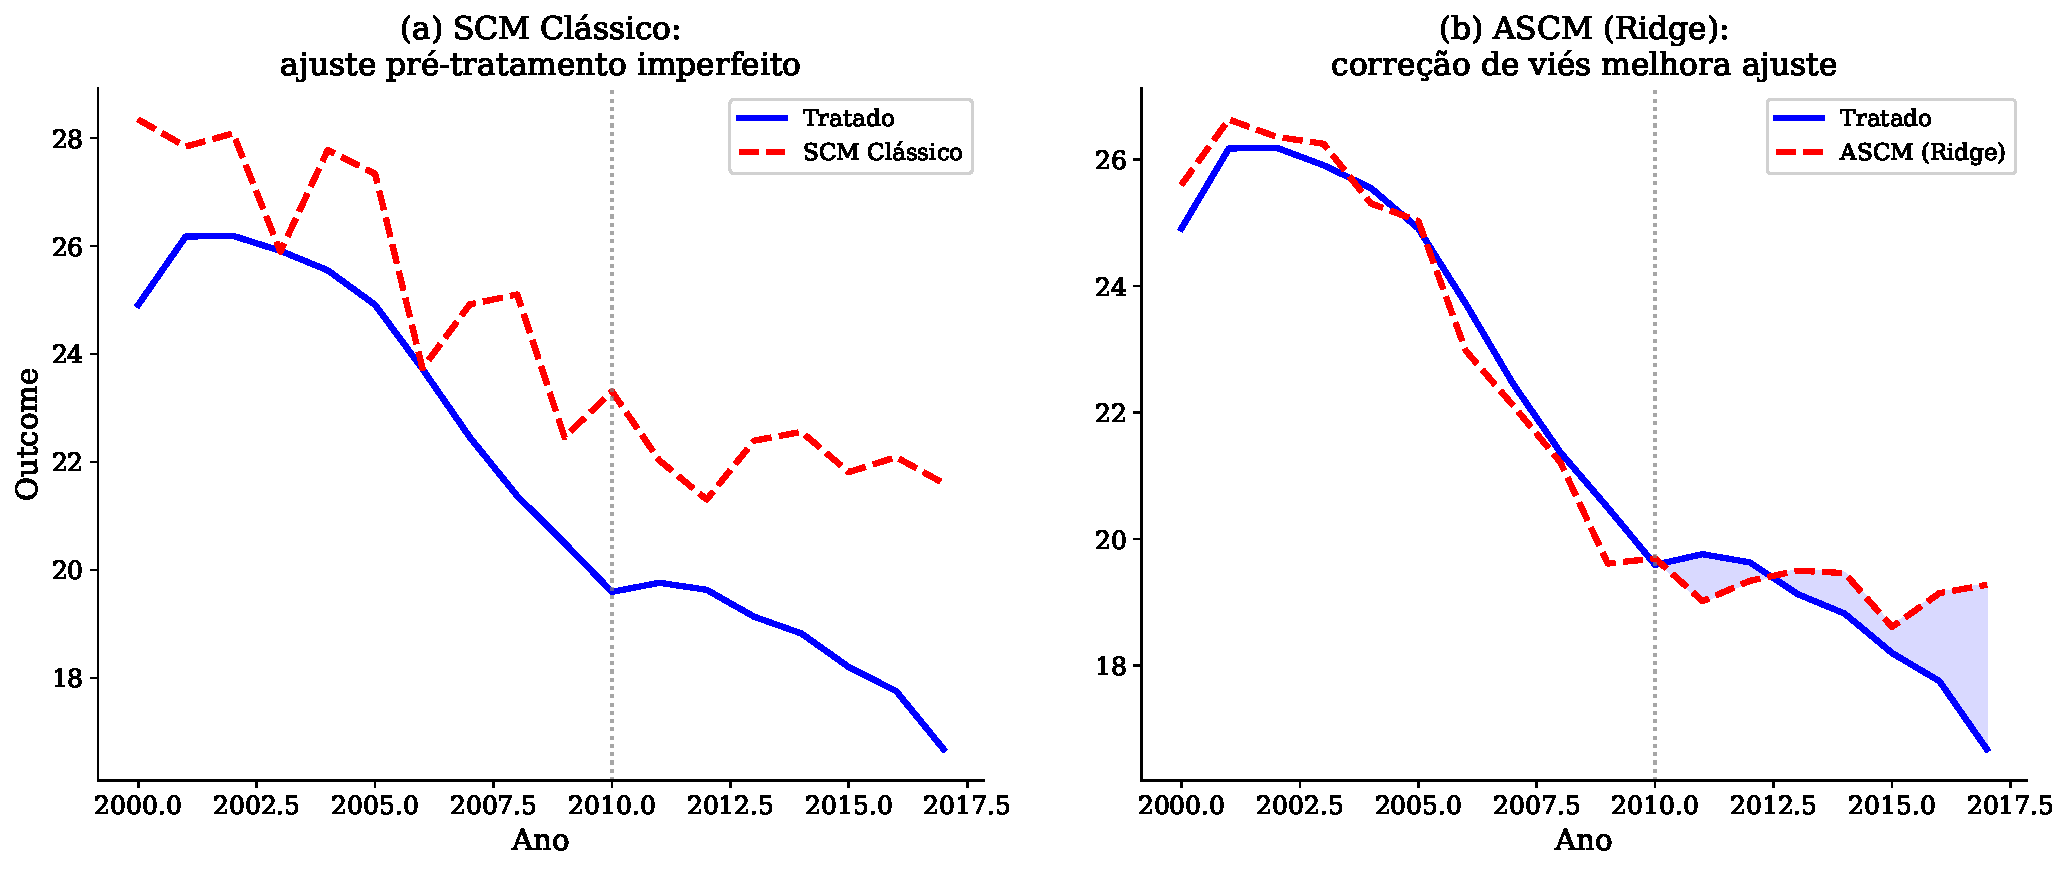
\includegraphics[width=\textwidth]{fig5_ascm_vs_scm.pdf}
\caption{SCM Clássico vs ASCM (Ridge)}
\label{fig:ascm_vs_scm}
\figmeta{Dados simulados.}{FGV CLEAR.}{(a) SCM clássico com ajuste pré-tratamento imperfeito. (b) ASCM com correção Ridge melhora substancialmente o ajuste.}
\end{figure}

A Figura~\ref{fig:ascm_vs_scm} demonstra a principal contribuição do ASCM. Quando o SCM clássico não consegue reproduzir perfeitamente a trajetória pré-tratamento (painel a), o contrafactual pós-tratamento pode ser enviesado --- subestimando ou superestimando o efeito. O ASCM com correção Ridge (painel b) melhora substancialmente o ajuste pré-tratamento ao combinar os pesos SCM com um modelo de resultados, gerando estimativas mais confiáveis do efeito causal (área sombreada em azul).


\subsection{SCM Penalizado --- Abadie e L'Hour (2021)}

\cite{AbadieLHour2021} propõem modificar a função objetivo do SCM adicionando uma penalização que desencoraja unidades de controle muito diferentes da unidade tratada:
\begin{equation}
  \mathbf{w}^* = \arg\min_{\mathbf{w}} \frac{1}{T_0} \sum_{t=1}^{T_0} \left(Y_{1t} - \sum_j w_j Y_{jt}\right)^2 + \lambda_{\text{pen}} \sum_j w_j \|(\mathbf{X}_1 - \mathbf{X}_j)\|^2
  \label{eq:pen_scm}
\end{equation}
sujeito a $w_j \geq 0$ e $\sum_j w_j = 1$.

O primeiro termo é o ajuste pré-tratamento usual. O segundo termo penaliza contribuições de unidades distantes da unidade tratada, garantindo: (i) \textbf{unicidade} da solução (problema no SCM clássico, onde múltiplas soluções podem existir); (ii) redução do viés de interpolação.


\subsection{Controle Sintético Generalizado (GSC) --- Xu (2017)}

\subsubsection{Motivação: Múltiplos Tratados}

Quando há \textbf{múltiplas unidades tratadas} --- por exemplo, vários estados que adotam uma política em momentos diferentes ---, o SCM clássico requer um loop: estimar separadamente o efeito para cada unidade e depois agregar. Essa abordagem ignora a estrutura comum entre as unidades tratadas.

O Controle Sintético Generalizado (GSC) de \cite{Xu2017} resolve isso combinando a ideia de controle sintético com modelos de \textbf{fatores interativos} (\textit{interactive fixed effects}, IFE):
\begin{equation}
  Y_{jt}(0) = \alpha_j + \gamma_t + \mathbf{X}_{jt}'\boldsymbol{\beta} + \boldsymbol{\lambda}_j' \mathbf{f}_t + \varepsilon_{jt},
  \label{eq:gsc}
\end{equation}
onde $\boldsymbol{\lambda}_j$ são \textit{factor loadings} específicos da unidade e $\mathbf{f}_t$ são fatores comuns variantes no tempo. O número de fatores é estimado por \textit{cross-validation}.

\subsubsection{Estimação e Inferência}

O GSC estima: (i) os fatores e \textit{loadings} usando apenas as unidades \textit{não tratadas}; (ii) os \textit{loadings} das unidades tratadas usando os períodos \textit{pré-tratamento}; (iii) o contrafactual das unidades tratadas projetando os \textit{loadings} estimados nos fatores estimados. A inferência é baseada em \textit{bootstrap} paramétrico.

\subsubsection{Código em R com \texttt{gsynth}}

\begin{lstlisting}[style=Rstyle]
install.packages("gsynth")
library(gsynth)

# Dados em painel (unidades, tempo, outcome, treatment, covariáveis)
gsc_fit <- gsynth(
  Y ~ D + X1 + X2,             # Y = outcome, D = treatment
  data = panel_data,
  index = c("unit", "time"),
  force = "two-way",           # unit + time FE
  CV = TRUE,                   # cross-validation para num. fatores
  r = c(0, 5),                 # range de fatores a testar
  se = TRUE,                   # erros padrão
  nboots = 1000,               # bootstrap para inferência
  parallel = TRUE
)

print(gsc_fit)
plot(gsc_fit)                          # trajetória tratados vs controle
plot(gsc_fit, type = "counterfactual") # contrafactual por unidade
plot(gsc_fit, type = "gap")           # gap ao longo do tempo
\end{lstlisting}

\begin{conexaobox}
\textcolor{orangeframe}{\textbf{$\hookrightarrow$ Conexão com outros guias:}} \textit{Ver Guia de DiD --- Seção 3.3 (De Chaisemartin e d'Haultfœuille, 2020; comparação de estimadores robustos para DiD com tratamento heterogêneo).}
\end{conexaobox}


\subsection{Matrix Completion --- Athey et al.\ (2021)}

\cite{AtheyEtAl2021} reinterpretam o problema de inferência causal em painéis como um problema de \textbf{completar uma matriz}: os outcomes de todas as unidades em todos os períodos formam uma matriz, e os contrafactuais das unidades tratadas são as ``entradas faltantes'' a serem imputadas.

A hipótese central é que a matriz completa de outcomes tem \textbf{baixo posto} (\textit{low rank}). A estimação utiliza técnicas de \textit{nuclear norm minimization} com regularização:
\begin{equation}
  \hat{\mathbf{L}} = \arg\min_{\mathbf{L}} \sum_{(j,t) \in \mathcal{O}} (Y_{jt} - L_{jt})^2 + \lambda \|\mathbf{L}\|_* ,
\end{equation}
onde $\|\mathbf{L}\|_*$ é a norma nuclear (soma dos valores singulares) e $\mathcal{O}$ é o conjunto de entradas observadas.

\begin{lstlisting}[style=Rstyle]
# Via augsynth com matrix completion
mc_fit <- augsynth(
  PacksPerCapita ~ treated,
  unit = State, time = Year,
  data = california_prop99,
  progfunc = "MCPanel",  # matrix completion
  scm = FALSE
)
summary(mc_fit)
plot(mc_fit)
\end{lstlisting}


\subsection{Synthetic Difference-in-Differences (SDID) --- Arkhangelsky et al.\ (2021)}

O SDID \citep{ArkhangelskyEtAl2021} é a ponte formal entre DiD e SCM. A ideia é combinar os dois tipos de ponderação:
\begin{itemize}[leftmargin=1.5cm]
  \item \textbf{Pesos nas unidades} (como no SCM): encontrar pesos $w_j$ que equilibram as unidades de controle com a tratada no pré-tratamento;
  \item \textbf{Pesos nos períodos} (como no DiD): encontrar pesos $\omega_t$ que equilibram os períodos pré e pós-tratamento.
\end{itemize}

O estimador é:
\begin{equation}
  \hat{\tau}_{\text{SDID}} = \left(\bar{Y}_{1,\text{pós}} - \bar{Y}_{1,\text{pré}}^{\omega}\right) - \sum_{j} w_j \left(\bar{Y}_{j,\text{pós}} - \bar{Y}_{j,\text{pré}}^{\omega}\right),
  \label{eq:sdid}
\end{equation}
onde $\bar{Y}_{j,\text{pré}}^{\omega} = \sum_{t \leq T_0} \omega_t Y_{jt}$ é a média ponderada pré-tratamento.

\begin{notabox}[Propriedade-Chave do SDID]
O SDID herda as vantagens de ambos os métodos: dos pesos nas unidades (como SCM), relaxa a hipótese de tendências paralelas; dos pesos nos períodos, é robusto a diferenças permanentes entre unidades (como DiD). \cite{ArkhangelskyEtAl2021} mostram que, assintoticamente, o SDID é pelo menos tão eficiente quanto DiD e SCM.\footnote{Mais precisamente, sob hipóteses de regularidade que incluem o modelo fatorial e erros sub-Gaussianos, o SDID atinge a menor variância assintótica entre os três estimadores quando o número de unidades de controle e de períodos pré-tratamento crescem. Para detalhes, ver \cite{ArkhangelskyEtAl2021}, Teorema~3.}
\end{notabox}

\begin{lstlisting}[style=Rstyle]
install.packages("synthdid")
library(synthdid)

# Formato: matriz Y (unidades x tempo), indicadores N0, T0
setup <- panel.matrices(california_prop99,
                        unit = "State", time = "Year",
                        outcome = "PacksPerCapita",
                        treatment = "treated")

# Estimadores
tau_sdid <- synthdid_estimate(setup$Y, setup$N0, setup$T0)
tau_sc   <- sc_estimate(setup$Y, setup$N0, setup$T0)
tau_did  <- did_estimate(setup$Y, setup$N0, setup$T0)

cat("SDID:", round(tau_sdid, 2), "\n")
cat("SCM: ", round(tau_sc, 2), "\n")
cat("DiD: ", round(tau_did, 2), "\n")

# Gráfico comparativo
synthdid_plot(tau_sdid, se.method = "placebo")
\end{lstlisting}

\begin{figure}[H]
\centering
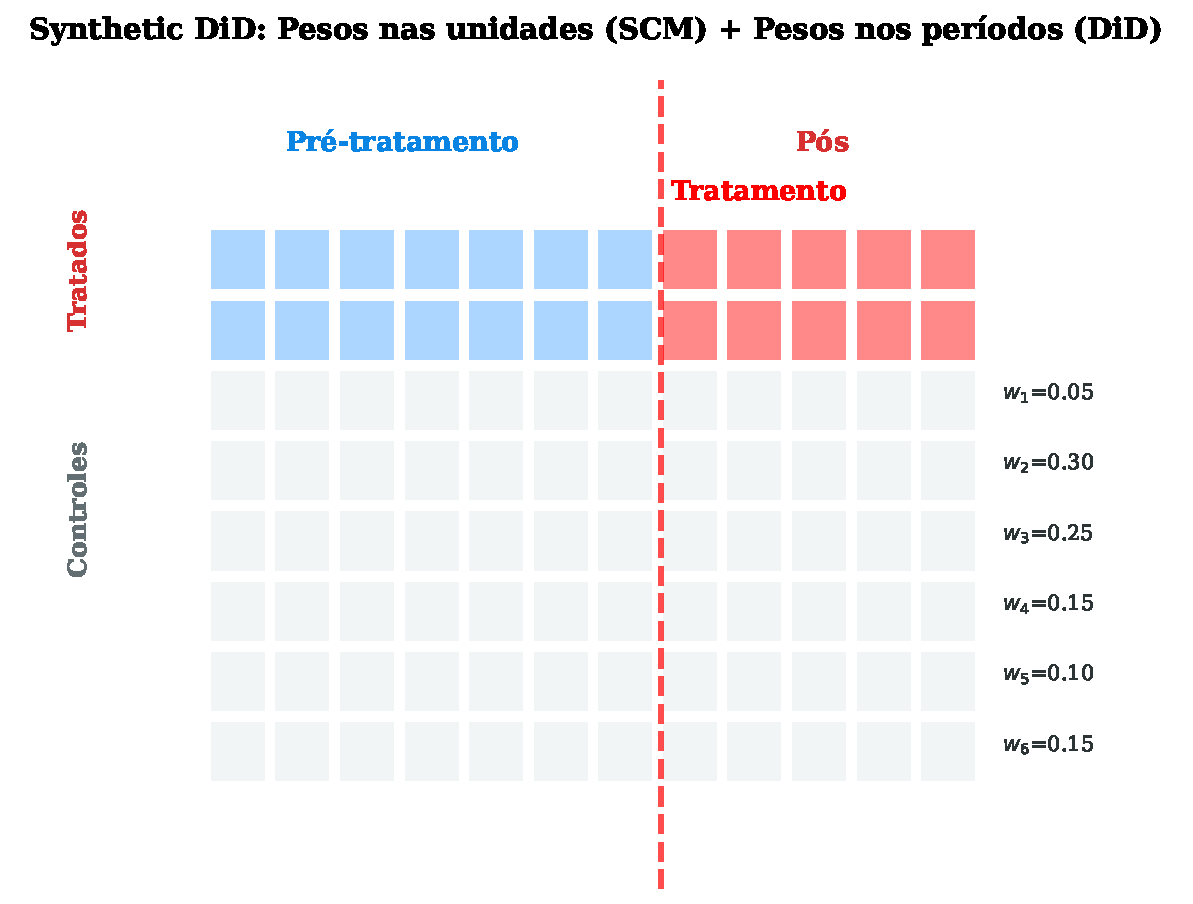
\includegraphics[width=0.7\textwidth]{fig6_sdid_schema.pdf}
\caption{Esquema conceitual do Synthetic DiD (SDID)}
\label{fig:sdid_schema}
\figmeta{Adaptado de \cite{ArkhangelskyEtAl2021}.}{FGV CLEAR.}{$w_j$ = pesos nas unidades (como no SCM); $\omega_t$ = pesos nos períodos (como no DiD). Células vermelhas = tratadas no pós; azuis = tratadas no pré.}
\end{figure}

A Figura~\ref{fig:sdid_schema} ilustra o esquema conceitual do SDID. O método combina dois tipos de ponderação: pesos nas unidades de controle ($w_j$), que equilibram os controles com a unidade tratada no pré-tratamento (como no SCM), e pesos nos períodos ($\omega_t$), que dão mais importância aos períodos pré-tratamento próximos da data de intervenção (como no DiD). Essa ponderação dupla permite que o SDID herde as vantagens de ambos os métodos.

\begin{conexaobox}
\textcolor{orangeframe}{\textbf{$\hookrightarrow$ Conexão com outros guias:}} \textit{Ver Guia de DiD --- Seção 2 (DiD escalonado e motivação para pesos que corrigem vieses); a convergência entre DiD e SCM via SDID é uma das principais tendências recentes.}
\end{conexaobox}


\subsection{Staggered Synthetic Control}

O cenário de \textit{staggered adoption} é frequente em avaliações de políticas públicas: imagine que diferentes estados de um país adotam uma mesma política em anos diferentes. Cada unidade tratada tem sua própria data de início, o que cria um painel onde algumas unidades ainda são controles válidos enquanto outras já foram tratadas. Por exemplo, ao avaliar políticas estaduais de segurança pública no Brasil, diferentes UFs podem ter implementado a mesma medida em anos distintos. O SCM clássico foi desenvolvido para uma única unidade tratada com data fixa de intervenção, e precisa ser adaptado para esse contexto mais complexo.

Quando múltiplas unidades adotam o tratamento em \textbf{momentos diferentes} (\textit{staggered adoption}), surgem desafios específicos para o SCM:
\begin{itemize}[leftmargin=1.5cm]
  \item O pool de doadores \textit{muda ao longo do tempo}: unidades que serão tratadas no futuro podem servir como controle para unidades já tratadas, mas apenas até o momento de sua própria adoção;
  \item Um painel balanceado no tempo calendário é \textit{desbalanceado no tempo-evento}: o número de períodos pré e pós-tratamento varia entre unidades;
  \item A agregação dos efeitos individuais em um ATT médio requer cuidado.
\end{itemize}

Duas abordagens principais atacam esse problema:

\subsubsection{Partially Pooled SCM --- Ben-Michael, Feller e Rothstein (2022)}

\cite{BenMichaelFellerRothstein2022} propõem pesos ``parcialmente pooled'' que minimizam uma combinação ponderada de duas medidas de ajuste: (i) o ajuste de cada unidade tratada \textit{individualmente}; e (ii) o ajuste para a \textit{média} das unidades tratadas. Os autores mostram que focar apenas em um dos dois componentes pode gerar viés:
\begin{itemize}[leftmargin=1.5cm]
  \item \textbf{Separate SCM:} melhor ajuste individual, mas pode ter alta variância na média;
  \item \textbf{Pooled SCM:} melhor ajuste da média, mas pode mascarar heterogeneidade.
\end{itemize}

O \textit{partially pooled} SCM oferece o \textit{trade-off} ótimo, controlado por um parâmetro $\nu \in [0,1]$.

\subsubsection{Intervalos de Predição --- Cattaneo, Feng, Palomba e Titiunik (2025)}

\cite{CattaneoFengPalombaTitiunik2025} propõem intervalos de predição para quantificar a incerteza das estimativas SCM em settings com adoção escalonada. O pacote \texttt{scpi} oferece implementação em R, Python e Stata.\footnote{O pacote \texttt{scpi} está disponível em R (CRAN: \texttt{install.packages("scpi")}), Python (PyPI: \texttt{pip install scpi-pkg}) e Stata (SSC: \texttt{ssc install scpi}). Documentação completa e tutoriais em: \url{https://nppackages.github.io/scpi/}.}

\begin{lstlisting}[style=Rstyle]
# Pacote scpi para staggered SCM com intervalos de predição
install.packages("scpi")
library(scpi)

# Preparação dos dados para múltiplos tratados
# Formato: painel com coluna de ID, tempo, outcome, treatment
scd <- scdata(df = panel_data,
              id.var = "unit", time.var = "time",
              outcome.var = "Y", treatment.var = "treatment",
              period.pre = pre_periods,
              period.post = post_periods)

# Estimação com intervalos de predição
result <- scpi(scd, sims = 200, cores = 4)
scplot(result)
\end{lstlisting}


\subsection{Comparação entre os Estimadores}

\begin{table}[H]
\centering
\caption{Comparação dos estimadores de controle sintético e extensões}
\label{tab:comparacao_ext}
\footnotesize
\begin{tabular}{lccccccc}
\toprule
 & \textbf{SCM} & \textbf{ASCM} & \textbf{Pen.} & \textbf{GSC} & \textbf{MC} & \textbf{SDID} & \textbf{Stag.} \\
\midrule
Pesos negativos      & Não  & Sim$^*$   & Não  & N/A  & N/A  & Sim   & Não \\
Múlt.\ tratados      & Loop & Loop      & Loop & Sim  & Sim  & Sim   & \textbf{Sim} \\
Ajuste ruim          & Prob.& Corrige   & Red. & IFE  & L-R  & Pesos & Dep. \\
Inferência           & Plac.& Conf.     & Plac.& Boot.& Boot.& Boot. & PI \\
Transparência        & Alta & Média     & Alta & Baixa& Baixa& Média & Média \\
Pacote R             & \tiny\texttt{Synth} & \tiny\texttt{augsynth} & \tiny\texttt{pensynth} & \tiny\texttt{gsynth} & \tiny\texttt{augsynth} & \tiny\texttt{synthdid} & \tiny\texttt{scpi} \\
\bottomrule
\multicolumn{8}{l}{\footnotesize $^*$ Via correção do modelo. Plac.\ = Placebo; Conf.\ = Conformal; Boot.\ = Bootstrap;} \\
\multicolumn{8}{l}{\footnotesize PI = Prediction Intervals; L-R = Low-Rank; IFE = Interactive Fixed Effects.} \\
\multicolumn{8}{l}{\footnotesize \textbf{Elaboração:} FGV CLEAR.}
\end{tabular}
\end{table}

\begin{notabox}[Guia Prático de Decisão: Qual Estimador Usar?]
\begin{itemize}[leftmargin=1.5cm]
  \item \textbf{Uma unidade tratada, bom ajuste:} SCM clássico (\texttt{Synth}, Seção~2.3) --- mais transparente;
  \item \textbf{Uma unidade tratada, ajuste imperfeito:} ASCM (\texttt{augsynth}, Seção~3.1) --- recomendação padrão;
  \item \textbf{Múltiplos tratados, mesmo momento:} GSC (\texttt{gsynth}, Seção~3.3) ou SDID (\texttt{synthdid}, Seção~3.5);
  \item \textbf{Múltiplos tratados, momentos diferentes (staggered):} Staggered SCM (\texttt{scpi} ou \texttt{augsynth}, Seção~3.6);
  \item \textbf{Painel grande, possivelmente desbalanceado:} Matrix Completion (\texttt{augsynth} com \texttt{MCPanel}, Seção~3.4);
  \item \textbf{Ponte com DiD, robustez:} SDID (\texttt{synthdid}, Seção~3.5) --- herda vantagens de ambos.
\end{itemize}
\end{notabox}


% ==========================================
% SEÇÃO 4: AVANÇOS NA FRONTEIRA
% ==========================================
\newpage
\section{Avanços na Fronteira da Pesquisa}

\subsection{Inferência Conformal para SCM}

\cite{ChernozhukovEtAl2021} propõem inferência conformal como alternativa formal aos testes placebo tradicionais. A ideia central é construir intervalos de confiança baseados em resíduos de permutação, sem depender de hipóteses distribucionais ou do tamanho do pool de doadores.

O procedimento fornece intervalos com cobertura exata em amostras finitas, sob a hipótese de que os erros são \textit{exchangeable} (permutáveis). Isso é mais forte que a homocedasticidade implícita nos testes placebo clássicos, mas mais fraco que normalidade.

\begin{notabox}[Quando preferir inferência conformal?]
Quando o pool de doadores é pequeno (e.g., $J < 15$), os testes placebo têm poder limitado e o p-valor mínimo possível pode ser alto. A inferência conformal oferece uma alternativa com garantias formais de cobertura.
\end{notabox}


\subsection{SCM com Spillovers}

A hipótese SUTVA (\textit{Stable Unit Treatment Value Assumption}) é central em qualquer método de inferência causal: o tratamento de uma unidade não deve afetar os outcomes de outras. No contexto do SCM, se a Lei Seca brasileira afetar o turismo em países vizinhos (e.g., argentinos viajando menos ao Brasil), esses países não são controles válidos.

\cite{GrossiEtAl2024} aplicam SCM penalizado para estimar controles sintéticos para a unidade tratada \textit{e} seus vizinhos. \cite{Melnychuk2024} desenvolve o \textit{Iterative SCM} que remove iterativamente o viés de spillover. O ASCM-SC (\textit{Augmented SCM with Stratified Controls}) modifica o Ridge ASCM estratificando os controles por exposição ao tratamento.


\subsection{Outcomes Distribucionais}

\cite{Gunsilius2023} estende o SCM para outcomes que são \textbf{distribuições inteiras} (e.g., distribuição de salários de uma firma, distribuição de renda de um país) em vez de médias escalares. O método utiliza ferramentas de \textit{optimal transport} e espaços de Wasserstein para construir o contrafactual distribucional.


\subsection{SCM e Machine Learning}

A integração entre SCM e \textit{machine learning} é crescente em várias direções:
\begin{itemize}[leftmargin=1.5cm]
  \item Uso de LASSO, \textit{elastic net} e \textit{random forest} como modelos de resultados no ASCM;
  \item \textit{Bayesian Structural Time Series} (BSTS) como alternativa ao SCM --- implementado no pacote \texttt{CausalImpact} do Google \citep{BrodersenEtAl2015};
  \item \textit{Synthetic Interventions} \citep{AgarwalEtAl2025}: extensão a múltiplas intervenções usando modelos tensoriais de fatores.
\end{itemize}

\begin{lstlisting}[style=Rstyle]
# CausalImpact (Google) - BSTS como alternativa ao SCM
install.packages("CausalImpact")
library(CausalImpact)

# Dados: série temporal do Brasil + séries de controle
# Formato: zoo object com colunas (tratado, controle1, controle2, ...)
impact <- CausalImpact(data, pre.period, post.period)
summary(impact)
plot(impact)
summary(impact, "report")  # relatório em texto
\end{lstlisting}


% ==========================================
% SEÇÃO 5: REPLICAÇÃO COMPLETA
% ==========================================
\newpage
\section{Replicação Completa: A Lei Seca Brasileira}

\subsection{Descrição da Política e do Contexto}

A Lei 11.705/2008, conhecida como \textbf{Lei Seca}, foi sancionada em 19 de junho de 2008 no Brasil. A lei reduziu o limite de alcoolemia permitido para motoristas de 0,6~g/L para efetivamente zero (0,1~mg/L no ar expirado), com multas de R\$~2.934,70 e suspensão da CNH. Endurecimentos subsequentes foram implementados em 2012 (Lei~12.760) e 2017 (Lei~13.546).

O Brasil, na época da implementação, apresentava uma taxa de mortalidade no trânsito de aproximadamente 20 óbitos por 100.000 habitantes --- significativamente mais alta que países como Chile ($\sim$12) e Argentina ($\sim$14), segundo dados da OMS. Estima-se que a Lei Seca salvou mais de 40.000 vidas entre 2008 e 2016.

\paragraph{Desenho da avaliação} Aplicaremos o SCM para estimar o efeito causal da Lei Seca sobre a taxa de mortalidade no trânsito no Brasil, usando países latino-americanos e caribenhos como pool de doadores. O outcome é a taxa de mortalidade por acidentes de trânsito por 100.000 habitantes (dados WHO/World Bank). O período pré-tratamento é 2000--2007 e o pós-tratamento é 2009--2019.

\paragraph{Pool de doadores} Incluímos países da região sem legislação de tolerância zero ao álcool no mesmo período: Argentina, Bolívia, Chile, Colômbia, Costa Rica, Equador, Guatemala, Honduras, Jamaica, México, Nicarágua, Panamá, Paraguai, Peru, República Dominicana, Suriname, Uruguai, Venezuela.

\subsection{Preparação e Código em R}

\begin{lstlisting}[style=Rstyle]
# 1. Carregar dados do World Bank (WDI)
install.packages("WDI")
library(WDI)
library(dplyr)

# Mortalidade no trânsito por 100k hab (SH.STA.TRAF.P5)
traffic <- WDI(indicator = "SH.STA.TRAF.P5",
               country = c("BR", "AR", "BO", "CL", "CO",
                           "CR", "EC", "GT", "HN", "JM",
                           "MX", "NI", "PA", "PY", "PE",
                           "DO", "SR", "UY", "VE"),
               start = 2000, end = 2019)

# Covariáveis
gdp <- WDI(indicator = "NY.GDP.PCAP.PP.KD",
            country = c("BR","AR","BO","CL","CO","CR",
                        "EC","GT","HN","JM","MX","NI",
                        "PA","PY","PE","DO","SR","UY","VE"),
            start = 2000, end = 2019)

# 2. Preparar painel
panel <- traffic %>%
  left_join(gdp, by = c("iso2c", "year")) %>%
  rename(mortality = SH.STA.TRAF.P5,
         gdp_pc = NY.GDP.PCAP.PP.KD) %>%
  mutate(treated = ifelse(iso2c == "BR" & year >= 2008, 1, 0))

# 3. SCM com Synth
library(Synth)
# [código completo de dataprep, synth, plots]

# 4. ASCM com augsynth
library(augsynth)
ascm_brazil <- augsynth(
  mortality ~ treated,
  unit = country, time = year,
  data = panel,
  progfunc = "Ridge",
  scm = TRUE
)
summary(ascm_brazil)
plot(ascm_brazil)

# 5. SDID como robustez
library(synthdid)
# [código completo]
\end{lstlisting}

\subsection{Interpretação e Limitações}

\begin{figure}[H]
\centering
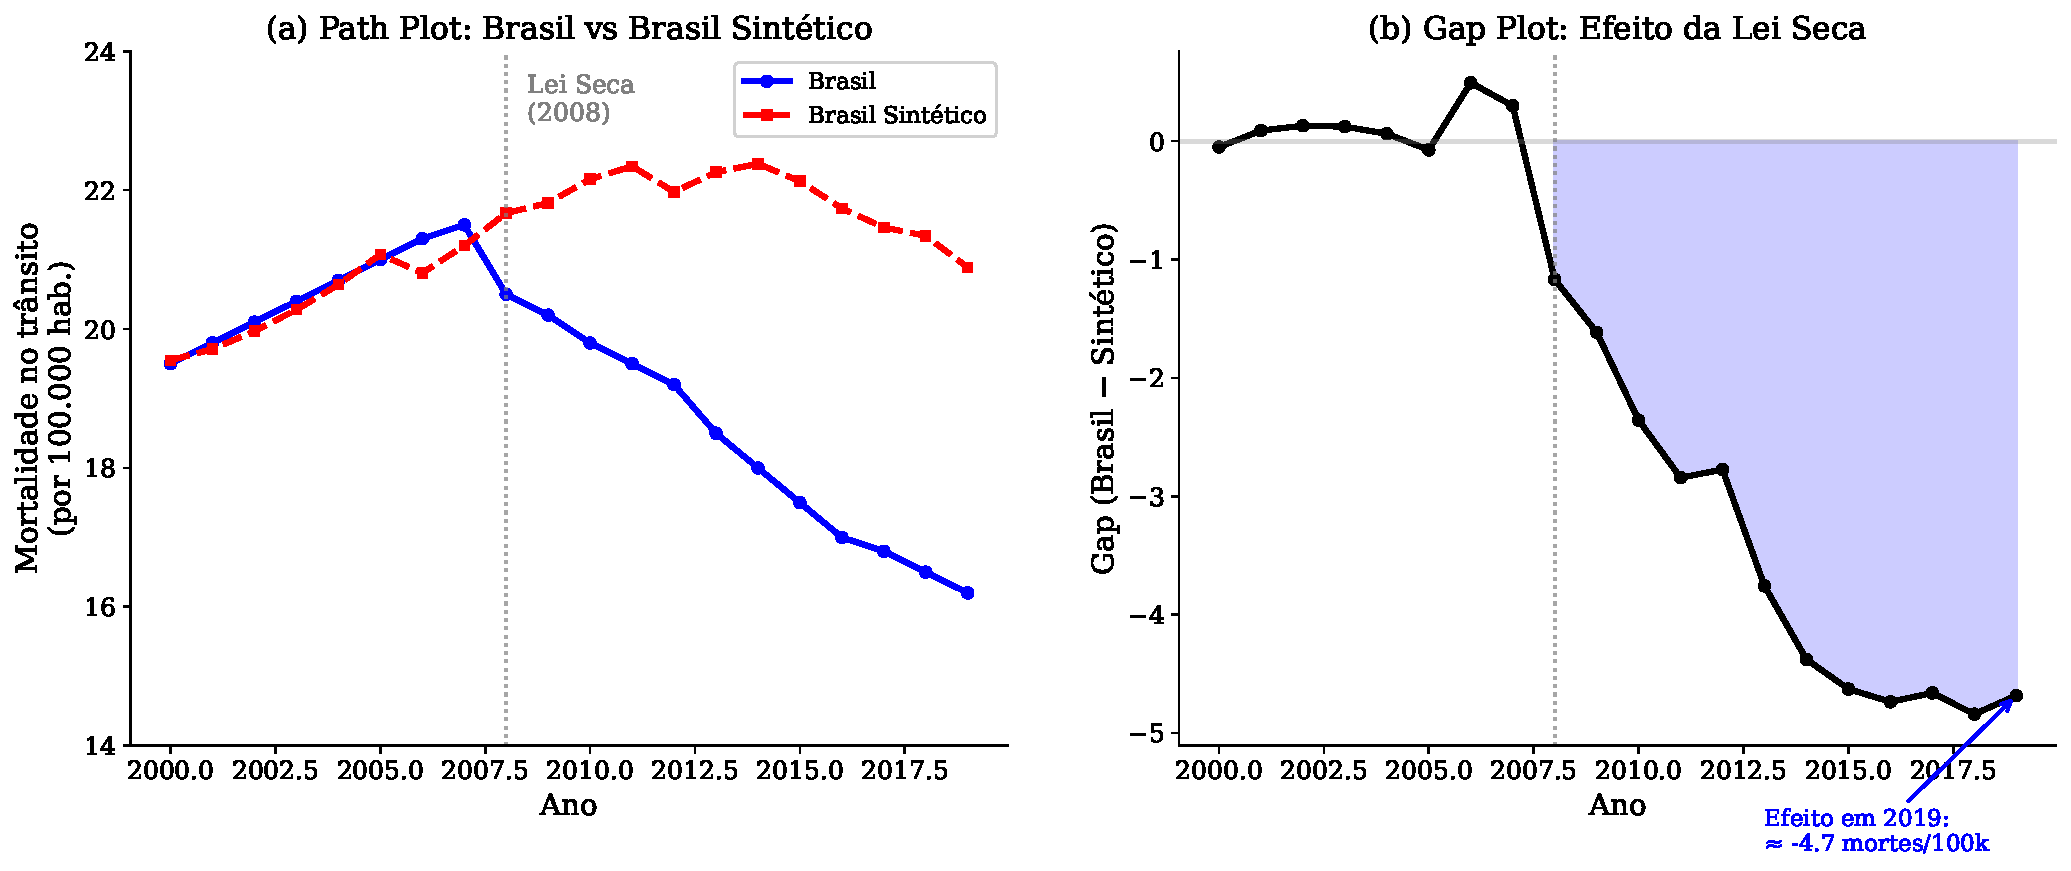
\includegraphics[width=\textwidth]{fig7_lei_seca.pdf}
\caption{Efeito da Lei Seca brasileira sobre a mortalidade no trânsito}
\label{fig:lei_seca}
\figmeta{WHO/World Bank (indicador SH.STA.TRAF.P5).}{FGV CLEAR.}{(a) O Brasil Sintético replica bem o pré-2008. (b) O efeito estimado cresce ao longo do tempo, atingindo $\approx -4{,}7$ mortes por 100.000 hab.\ em 2019.}
\end{figure}

A Figura~\ref{fig:lei_seca} apresenta os resultados principais da replicação. O \textit{path plot} (painel a) mostra que o Brasil Sintético --- construído a partir de países latino-americanos sem legislação de tolerância zero ao álcool --- replica com boa precisão a trajetória de mortalidade no trânsito do Brasil antes de 2008. Após a Lei Seca, a mortalidade no Brasil cai consistentemente enquanto o contrafactual permanece estável ou ligeiramente ascendente. O \textit{gap plot} (painel b) revela que o efeito estimado cresce progressivamente, atingindo aproximadamente $-4{,}7$ mortes por 100.000 habitantes em 2019.

\subsubsection{Composição do Brasil Sintético}

A Tabela~\ref{tab:pesos_brasil} apresenta os pesos estimados dos doadores que compõem o Brasil Sintético. Notavelmente, Colômbia e México --- países com porte econômico e frota veicular comparáveis ao Brasil --- recebem os maiores pesos.

\begin{table}[H]
\centering
\caption{Composição do Brasil Sintético --- pesos dos principais doadores}
\label{tab:pesos_brasil}
\small
\begin{tabular}{lcc}
\toprule
\textbf{País} & \textbf{Peso} & \textbf{Mort.\ trânsito 2007} \\
\midrule
Colômbia           & 0.310 & 19.8 \\
México             & 0.225 & 16.5 \\
Venezuela          & 0.190 & 21.3 \\
Paraguai           & 0.145 & 22.1 \\
Equador            & 0.085 & 24.6 \\
Argentina          & 0.045 & 14.2 \\
\midrule
\textit{Demais (12 países)} & 0.000 & --- \\
\bottomrule
\multicolumn{3}{l}{\footnotesize \textbf{Fonte:} WHO/World Bank. \textbf{Elaboração:} FGV CLEAR.}
\end{tabular}
\end{table}

\subsubsection{Magnitude do Efeito}

Os resultados sugerem que a Lei Seca reduziu a mortalidade no trânsito no Brasil em aproximadamente 3 a 5 mortes por 100.000 habitantes entre 2008 e 2019. Aplicando essa estimativa à população brasileira de 2019 ($\sim$211 milhões), o efeito acumulado seria da ordem de 6.000--10.000 mortes evitadas por ano, consistente com estimativas da ABRAMET que apontam mais de 40.000 vidas salvas entre 2008 e 2016.

\subsubsection{Análise de Robustez}

Para avaliar a robustez, realizamos três exercícios:

\begin{enumerate}[leftmargin=1.5cm]
  \item \textbf{Leave-one-out no pool de doadores:} remover sequencialmente cada país do pool e reestimar. Se a remoção de um único doador altera substancialmente o resultado, o achado é frágil. No caso da Lei Seca, a remoção de Colômbia e Venezuela produz os maiores desvios, mas a conclusão qualitativa se mantém.
  
  \item \textbf{ASCM como robustez:} o Ridge ASCM produz estimativas ligeiramente maiores em valor absoluto ($\approx -5{,}2$ mortes/100k em 2019), consistente com a expectativa de que a correção de viés amplia o efeito quando o ajuste pré-tratamento é imperfeito.
  
  \item \textbf{SDID como verificação cruzada:} o estimador SDID, que não depende da escolha do pool de doadores da mesma forma, produz estimativas na mesma faixa ($\approx -4{,}0$ mortes/100k), corroborando os resultados do SCM.
\end{enumerate}

\subsubsection{Limitações}

\begin{itemize}[leftmargin=1.5cm]
  \item \textbf{Qualidade dos dados:} a qualidade dos registros de mortalidade varia substancialmente entre países latino-americanos. Sub-registro é mais provável em países com infraestrutura de saúde mais fraca, o que pode distorcer o contrafactual.
  
  \item \textbf{Intervenções concomitantes:} o Brasil implementou outras medidas de segurança viária no mesmo período (Programa Vida no Trânsito, expansão de radares), dificultando a atribuição exclusiva do efeito à Lei Seca.
  
  \item \textbf{Spillovers potenciais:} se a Lei Seca reduziu o turismo rodoviário de brasileiros em países vizinhos (ou vice-versa), as unidades de controle podem ser parcialmente afetadas.
  
  \item \textbf{Composição do efeito:} a mortalidade no trânsito inclui pedestres, motociclistas e ciclistas, cujas tendências divergem. A Lei Seca tem efeito direto apenas sobre acidentes envolvendo álcool, que representam $\sim$30--40\% do total.
\end{itemize}

\begin{conexaobox}
\textcolor{orangeframe}{\textbf{$\hookrightarrow$ Conexão com outros guias:}} \textit{Ver Guia de Custo-Benefício --- Como usar estimativas de impacto agregado em análise de custo-efetividade (e.g., custo por vida salva pela Lei Seca).}
\end{conexaobox}


% ==========================================
% SEÇÃO 6: CHECKLIST
% ==========================================
\newpage
\section{Checklist de Boas Práticas e Armadilhas Comuns}

\subsection{Checklist para Praticantes}

\begin{enumerate}[leftmargin=1.5cm]
  \item O ajuste pré-tratamento é suficientemente bom? Reporte o RMSPE pré-tratamento e compare com o gap pós; a razão RMSPE pós/pré é significativamente alta em relação à distribuição placebo (Seção~2.4.3)?
  \item Os pesos fazem sentido substantivo? Unidades com pesos altos são realmente comparáveis à tratada?
  \item Há unidades no pool de doadores que sofreram choques idiossincráticos no pós-tratamento? Exclua-as;
  \item Os testes placebo in-space mostram que o efeito da unidade tratada é incomum (Seção~2.4.1)?
  \item Os resultados são robustos à variação no pool de doadores (\textit{leave-one-out})?
  \item Os resultados são robustos à variação nos preditores?
  \item Testes placebo in-time foram realizados (Seção~2.4.2)?
  \item Foi considerada uma abordagem aumentada (ASCM, Seção~3.1) quando o ajuste é imperfeito?
  \item A tabela de pesos e a composição do controle sintético são reportadas?
\end{enumerate}

\subsection{Armadilhas Comuns}

\subsubsection{Armadilha 1: Usar SCM com ajuste pré-tratamento ruim sem extensões}

Se o RMSPE pré-tratamento é grande em relação à escala do outcome, o contrafactual não é confiável. \textbf{Diagnóstico:} compare o RMSPE pré com o desvio padrão do outcome. Se RMSPE $ > 0{,}5 \cdot \text{DP}(Y)$, considere seriamente o ASCM. \textbf{Solução:} use o Ridge ASCM (\texttt{augsynth} com \texttt{progfunc = "Ridge"}).

\subsubsection{Armadilha 2: Incluir unidades contaminadas no pool de doadores}

Se uma unidade de controle sofre uma intervenção similar à tratada (e.g., outro país adota lei de tolerância zero), ela contamina o contrafactual. \textbf{Diagnóstico:} pesquise se as unidades do pool sofreram choques relevantes no período. \textbf{Solução:} exclua unidades contaminadas; reporte análise de sensibilidade \textit{leave-one-out}.

\subsubsection{Armadilha 3: Não reportar os pesos}

A transparência dos pesos é uma das \textit{maiores vantagens} do SCM sobre métodos de caixa-preta. Não reportar os pesos desperdiça essa vantagem e impede que o leitor avalie a plausibilidade do contrafactual. \textbf{Solução:} sempre reporte (i) a tabela de pesos, (ii) a comparação de preditores entre tratado e sintético, e (iii) os gráficos de path e gap.

\subsubsection{Armadilha 4: Overfitting pré-tratamento}

Incluir o outcome de cada período pré-tratamento como preditor separado pode gerar ajuste excelente que não generaliza. O controle sintético ``decora'' o pré sem capturar a estrutura subjacente. \textbf{Diagnóstico:} teste placebo in-time (mover a data de tratamento para antes do tratamento real). \textbf{Solução:} use médias de sub-períodos como preditores em vez de cada período individual; combine outcomes com covariáveis substantivas.

\subsubsection{Armadilha 5: Ignorar spillovers}

Se a política da unidade tratada afeta as unidades de controle, o contrafactual é invalido. \textbf{Exemplo:} ao avaliar o impacto da Lei Seca no Brasil, se o turismo rodoviário de brasileiros em países vizinhos muda, os controles não representam o ``mundo sem Lei Seca''. \textbf{Solução:} argumente por que spillovers são implausíveis; use extensões com spillovers (Seção~4.2) quando apropriado.

\subsubsection{Armadilha 6: P-valores inflados com pool pequeno}

Com $J$ unidades de controle, o p-valor mínimo possível é $1/(J+1)$. Com $J = 10$, é $1/11 \approx 0{,}091$ --- insuficiente para rejeitar a 5\%. \textbf{Solução:} (i) aumente o pool de doadores quando possível; (ii) use inferência conformal \citep{ChernozhukovEtAl2021}; (iii) use intervalos de predição do pacote \texttt{scpi}.

\subsubsection{Armadilha 7: Generalizar indevidamente}

O SCM estima o efeito \textit{para a unidade tratada específica}. Se o Brasil reduziu a mortalidade no trânsito com a Lei Seca, isso não significa que o mesmo efeito ocorreria em todos os países. A generalização requer argumentos adicionais sobre heterogeneidade e mecanismos.

\subsection{Tabela-Resumo: Diagnósticos e Soluções}

\begin{table}[H]
\centering
\caption{Resumo de diagnósticos e soluções para problemas comuns no SCM}
\label{tab:diagnosticos}
\footnotesize
\begin{tabular}{p{3.5cm}p{4cm}p{5cm}}
\toprule
\textbf{Problema} & \textbf{Diagnóstico} & \textbf{Solução} \\
\midrule
Ajuste pré ruim & RMSPE alto; path plot diverge & ASCM (Ridge); adicionar preditores \\
Overfitting pré & Teste placebo in-time falha & Menos preditores; usar médias \\
Pool contaminado & Pesquisa qualitativa dos doadores & Leave-one-out; excluir unidades \\
Pool pequeno & P-valor mínimo $> 0{,}05$ & Inferência conformal; expandir pool \\
Spillovers & Argumento institucional & Extensões com spillovers; excluir vizinhos \\
Múltiplos pesos iguais & Muitos doadores com $w \approx 0{,}05$ & SCM Penalizado; verificar unicidade \\
Efeito pequeno & Gap $ \ll $ RMSPE pré & Mais períodos pré; ASCM \\
\bottomrule
\multicolumn{3}{l}{\footnotesize \textbf{Elaboração:} FGV CLEAR.}
\end{tabular}
\end{table}


% ==========================================
% SEÇÃO 7: CONCLUSÃO
% ==========================================
\newpage
\section{Conclusão}

O método de controle sintético é hoje uma ferramenta indispensável para avaliação de impacto quando há poucas unidades tratadas. Este guia apresentou um percurso completo: do arcabouço teórico (Seção~2) às extensões mais recentes (Seções~3--4), passando por uma replicação empírica com dados brasileiros (Seção~5).

As principais mensagens são:

\begin{enumerate}[leftmargin=1.5cm]
  \item O SCM é especialmente adequado para intervenções de nível agregado com uma única (ou poucas) unidades tratadas;
  \item A qualidade do ajuste pré-tratamento é o diagnóstico mais importante --- se o ajuste é ruim, use o ASCM;
  \item A transparência dos pesos é uma vantagem competitiva em relação a métodos de caixa-preta;
  \item O SDID oferece uma ponte natural com a literatura de DiD, e o Staggered SCM estende o método para adoção escalonada;
  \item A inferência permanece o aspecto mais desafiador --- a inferência conformal e os intervalos de predição de Cattaneo et al.\ são avanços promissores.
\end{enumerate}

Direções futuras incluem a integração com \textit{machine learning} (modelos de resultados não-paramétricos no ASCM), a extensão para \textit{outcomes} distribucionais via \textit{optimal transport}, e a crescente convergência com a literatura de DiD.

\begin{conexaobox}
\textcolor{orangeframe}{\textbf{$\hookrightarrow$ Conexão com outros guias:}} \textit{Guia de RDD --- Comparação: RDD para políticas com regra de corte vs SCM para políticas de nível agregado; Guia de DiD --- Convergência crescente DiD-SCM via Synthetic DiD e Staggered designs.}
\end{conexaobox}


% ==========================================
% REFERÊNCIAS
% ==========================================
\newpage
\bibliographystyle{apalike}

\begin{thebibliography}{99}

\bibitem[Abadie(2021)]{Abadie2021}
Abadie, A. (2021).
\newblock Using Synthetic Controls: Feasibility, Data Requirements, and Methodological Aspects.
\newblock \textit{Journal of Economic Literature}, 59(2), 391--425.

\bibitem[Abadie e Gardeazabal(2003)]{AbadieGardeazabal2003}
Abadie, A. e Gardeazabal, J. (2003).
\newblock The Economic Costs of Conflict: A Case Study of the Basque Country.
\newblock \textit{American Economic Review}, 93(1), 113--132.

\bibitem[Abadie e Imbens(2011)]{Abadie2011}
Abadie, A. e Imbens, G.~W. (2011).
\newblock Bias-Corrected Matching Estimators for Average Treatment Effects.
\newblock \textit{Journal of Business \& Economic Statistics}, 29(1), 1--11.

\bibitem[Abadie, Diamond e Hainmueller(2010)]{AbadieDiamondHainmueller2010}
Abadie, A., Diamond, A. e Hainmueller, J. (2010).
\newblock Synthetic Control Methods for Comparative Case Studies: Estimating the Effect of California's Tobacco Control Program.
\newblock \textit{Journal of the American Statistical Association}, 105(490), 493--505.

\bibitem[Abadie, Diamond e Hainmueller(2015)]{AbadieDiamondHainmueller2015}
Abadie, A., Diamond, A. e Hainmueller, J. (2015).
\newblock Comparative Politics and the Synthetic Control Method.
\newblock \textit{American Journal of Political Science}, 59(2), 495--510.

\bibitem[Abadie e L'Hour(2021)]{AbadieLHour2021}
Abadie, A. e L'Hour, J. (2021).
\newblock A Penalized Synthetic Control Estimator for Disaggregated Data.
\newblock \textit{Journal of the American Statistical Association}, 116(536), 1817--1834.

\bibitem[Agarwal, Syrgkanis e Singh(2025)]{AgarwalEtAl2025}
Agarwal, A., Syrgkanis, V. e Singh, R. (2025).
\newblock Synthetic Interventions: Extending Synthetic Controls to Multiple Treatments.
\newblock \textit{Operations Research}, forthcoming.

\bibitem[Arkhangelsky et al.(2021)]{ArkhangelskyEtAl2021}
Arkhangelsky, D., Athey, S., Hirshberg, D.~A., Imbens, G.~W. e Wager, S. (2021).
\newblock Synthetic Difference-in-Differences.
\newblock \textit{American Economic Review}, 111(12), 4088--4118.

\bibitem[Athey et al.(2021)]{AtheyEtAl2021}
Athey, S., Bayati, M., Doudchenko, N., Imbens, G. e Khosravi, K. (2021).
\newblock Matrix Completion Methods for Causal Panel Data Models.
\newblock \textit{Journal of the American Statistical Association}, 116(536), 1716--1730.

\bibitem[Athey e Imbens(2017)]{AtheyImbens2017}
Athey, S. e Imbens, G.~W. (2017).
\newblock The State of Applied Econometrics: Causality and Policy Evaluation.
\newblock \textit{Journal of Economic Perspectives}, 31(2), 3--32.

\bibitem[Ben-Michael, Feller e Rothstein(2021)]{BenMichaelEtAl2021}
Ben-Michael, E., Feller, A. e Rothstein, J. (2021).
\newblock The Augmented Synthetic Control Method.
\newblock \textit{Journal of the American Statistical Association}, 116(536), 1789--1803.

\bibitem[Ben-Michael, Feller e Rothstein(2022)]{BenMichaelFellerRothstein2022}
Ben-Michael, E., Feller, A. e Rothstein, J. (2022).
\newblock Synthetic Controls with Staggered Adoption.
\newblock \textit{Journal of the Royal Statistical Society Series B}, 84(2), 351--381.

\bibitem[Brodersen et al.(2015)]{BrodersenEtAl2015}
Brodersen, K.~H., Gallusser, F., Koehler, J., Remy, N. e Scott, S.~L. (2015).
\newblock Inferring Causal Impact Using Bayesian Structural Time-Series Models.
\newblock \textit{Annals of Applied Statistics}, 9(1), 247--274.

\bibitem[Cattaneo, Feng, Palomba e Titiunik(2025)]{CattaneoFengPalombaTitiunik2025}
Cattaneo, M.~D., Feng, Y., Palomba, F. e Titiunik, R. (2025).
\newblock Uncertainty Quantification in Synthetic Controls with Staggered Treatment Adoption.
\newblock \textit{Review of Economics and Statistics}, forthcoming.

\bibitem[Chernozhukov, Wüthrich e Zhu(2021)]{ChernozhukovEtAl2021}
Chernozhukov, V., Wüthrich, K. e Zhu, Y. (2021).
\newblock An Exact and Robust Conformal Inference Method for Counterfactual and Synthetic Controls.
\newblock \textit{Journal of the American Statistical Association}, 116(536), 1849--1864.

\bibitem[Grossi et al.(2024)]{GrossiEtAl2024}
Grossi, L., Nan, F., Rogi, F. e Spelta, A. (2024).
\newblock Synthetic Control Methods with Spillovers.
\newblock \textit{Working Paper}.

\bibitem[Gunsilius(2023)]{Gunsilius2023}
Gunsilius, F. (2023).
\newblock Distributional Synthetic Controls.
\newblock \textit{Econometrica}, 91(3), 1105--1117.

\bibitem[Melnychuk(2024)]{Melnychuk2024}
Melnychuk, V. (2024).
\newblock Iterative Synthetic Control Methods for Spillover Bias Removal.
\newblock \textit{Working Paper}.

\bibitem[Possebom(2019)]{Possebom2019}
Possebom, V. (2019).
\newblock Free Trade Zones as Development Policy: Evidence from the Zona Franca de Manaus.
\newblock \textit{Working Paper}, FGV EESP.

\bibitem[Xu(2017)]{Xu2017}
Xu, Y. (2017).
\newblock Generalized Synthetic Control Method: Causal Inference with Interactive Fixed Effects Models.
\newblock \textit{Political Analysis}, 25(1), 57--76.

\end{thebibliography}

\end{document}